\chapter{LORA}

The Internet of Things (IoT) is often referred to as a collection of objects connected to the Internet using wireless networks; these connected objects aim to collect and exchange information from their surroundings. IoT enables a connection between the physical and the digital worlds; that connection produces a massive amount of data that can be used for the optimization of resources and to improve the efficiency of existing systems. 
\newline

\begin{figure}
	\begin{center}
		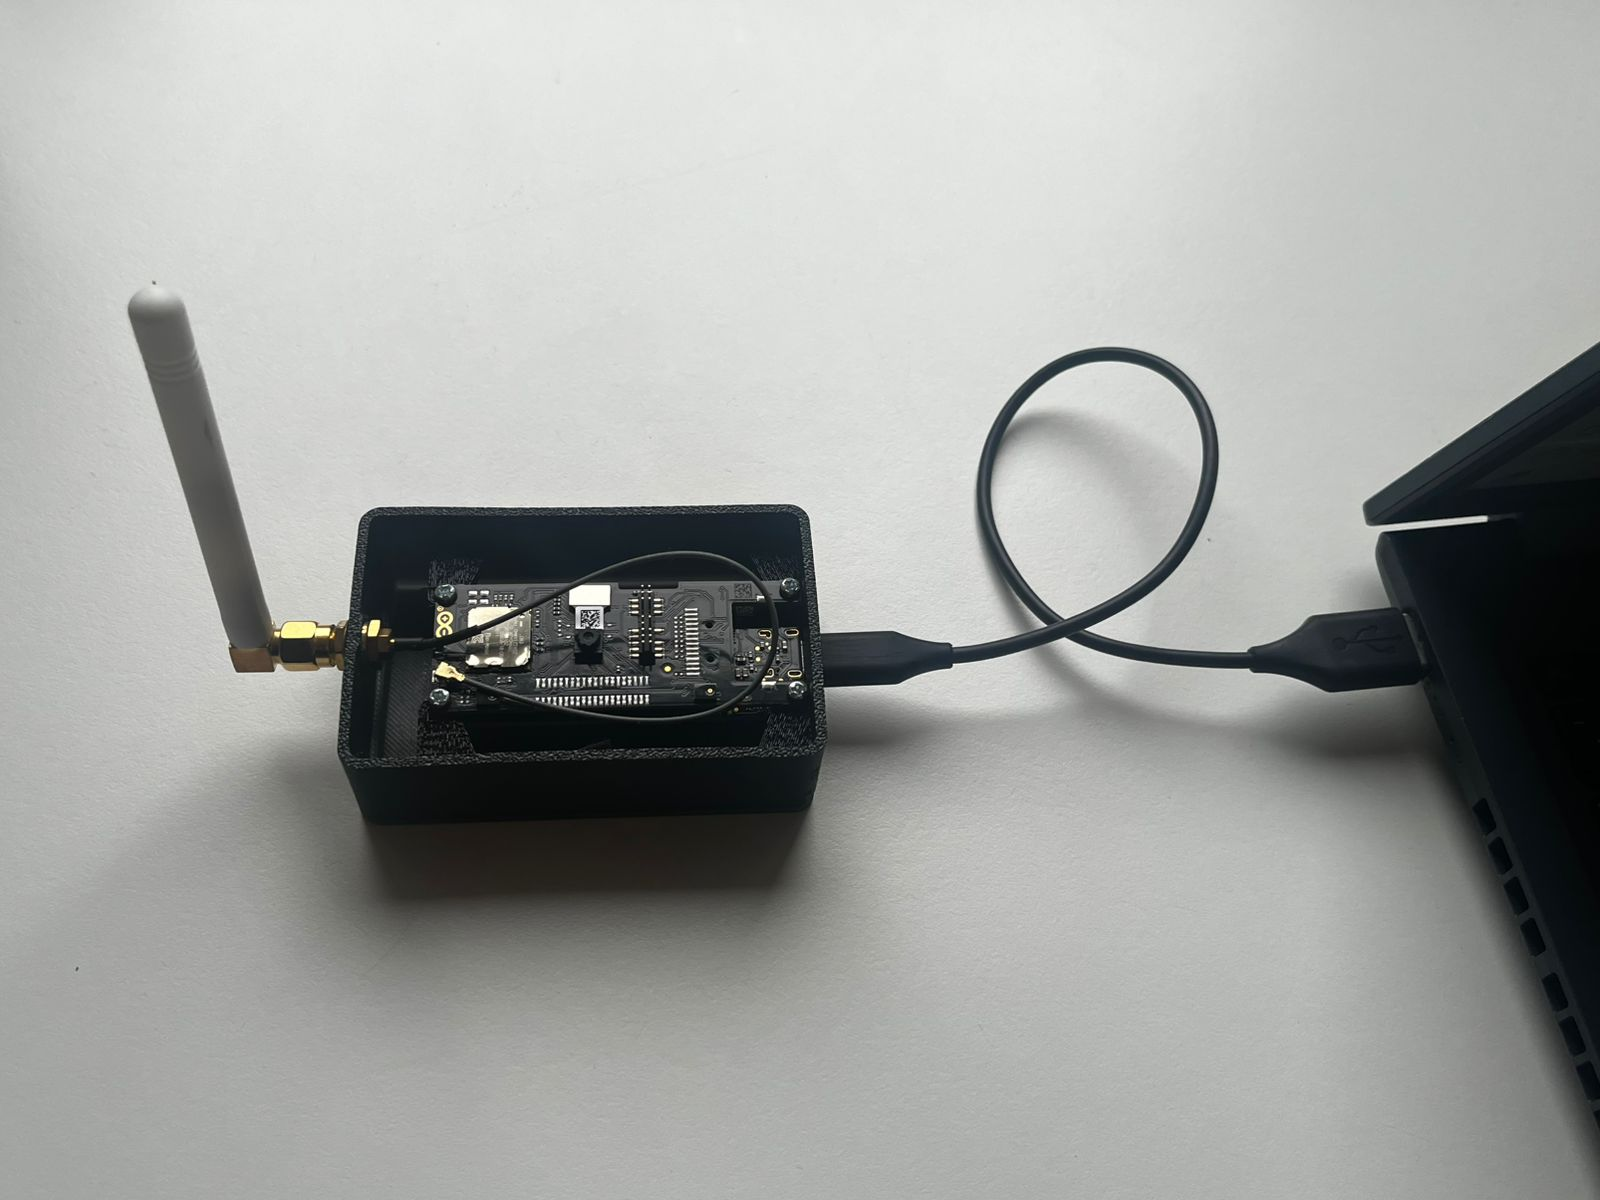
\includegraphics[width=0.7\linewidth]{Images/LORA/LORA1.jpg}
		\caption{LoRa}
		\label{LoRAWANRange} 
	\end{center}
\end{figure}

Many of the existing IoT devices will be connected to the Internet using short-range wireless networks such as Wi-Fi, Bluetooth, ZigBee, Z-Wave, etc. Cellular connections using networks such as 2G, 3G, and 4G will also connect IoT devices to the Internet. See Figure ~\ref{LoRAWANRange} for reference. Still, these short and medium-range wireless networks are not always suitable for IoT devices since they were developed for applications where power consumption and battery life are not significant issues. IoT devices usually have low-power consumption and send and receive low amounts of data.
\cite{ArduinoLoRaWAN101:2024}

\begin{figure}
	\begin{center}
		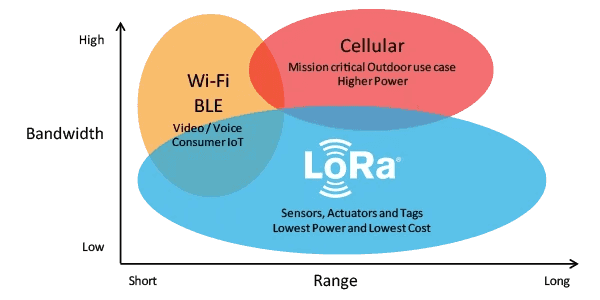
\includegraphics[width=0.7\linewidth]{Images/LORA/LoRAwanRange.png}
		\caption{Bandwidth vs. range of short distance, cellullar and LPWA networks. Image credits: The Things Network.}
		\label{LoRAWANRange} 
	\end{center}
\end{figure}

\section{Description}

\textbf{LoRa (Long Range)} is a wireless communication technology developed to facilitate long-distance, low-power data transmission, making it ideal for Internet of Things (IoT) applications. Utilizing the LoRa modulation technique, this technology enables devices to communicate over several kilometers with minimal energy consumption, which is essential for battery-powered devices deployed in remote or widespread locations. \cite{semtech_lora:2025}

\section{Key Features of LoRa}

\begin{itemize}
	\item \textbf{Long Range:} Capable of transmitting data over distances up to 15 kilometers in rural areas and 2-5 kilometers in urban settings. 
	\item \textbf{Low Power Consumption:} LoRa devices consume as little as 1-2 µA in sleep mode, around 20-50 mA during transmission, and can operate for 5-10 years on a standard battery. \cite{st_connectivity:2025}
	\item \textbf{Robustness:} Resistant to interference and capable of maintaining reliable communication in challenging environments by operating at a link budget of up to 168 dB. \cite{thethingsnetwork_lorawan:2025}
	\item \textbf{Scalability:} Supports large-scale deployments with thousands of devices interconnected within a single network. \cite{jooby_lora_features:2025}
\end{itemize}

\section{Hardware Components of the LoRa Implementation}

The LoRa implementation in the Portenta Vision Shield comprises several essential hardware components (Refer Figure ~\ref{tab:general-specifications}) that work together to enable seamless communication, data handling, and energy management. Below are the key components \cite{arduino_portenta:2025}.

\subsection{LoRa Transceiver Module}
\begin{itemize}
	\item \textbf{Function:} Provides radio communication using LoRa modulation for transmitting and receiving data \cite{semtech_sx1276:2025}.
	\item \textbf{Integrated Module:} The Vision Shield integrates the Murata CMWX1ZZABZ module, which is based on the Semtech SX1276 LoRa transceiver \cite{murata_transceiver:2025}.
	\item \textbf{Features:} 
	\begin{enumerate}
		\item Configurable frequency bands (868 MHz for Europe and 915 MHz for North America).
		\item Adjustable spreading factors for optimizing communication range and data rates.
		\item Supports adaptive data rates (ADR) to improve efficiency \cite{semtech_sx1276:2025}.
	\end{enumerate}
\end{itemize}

\subsection{Antenna}

\begin{figure}
	\begin{center}
		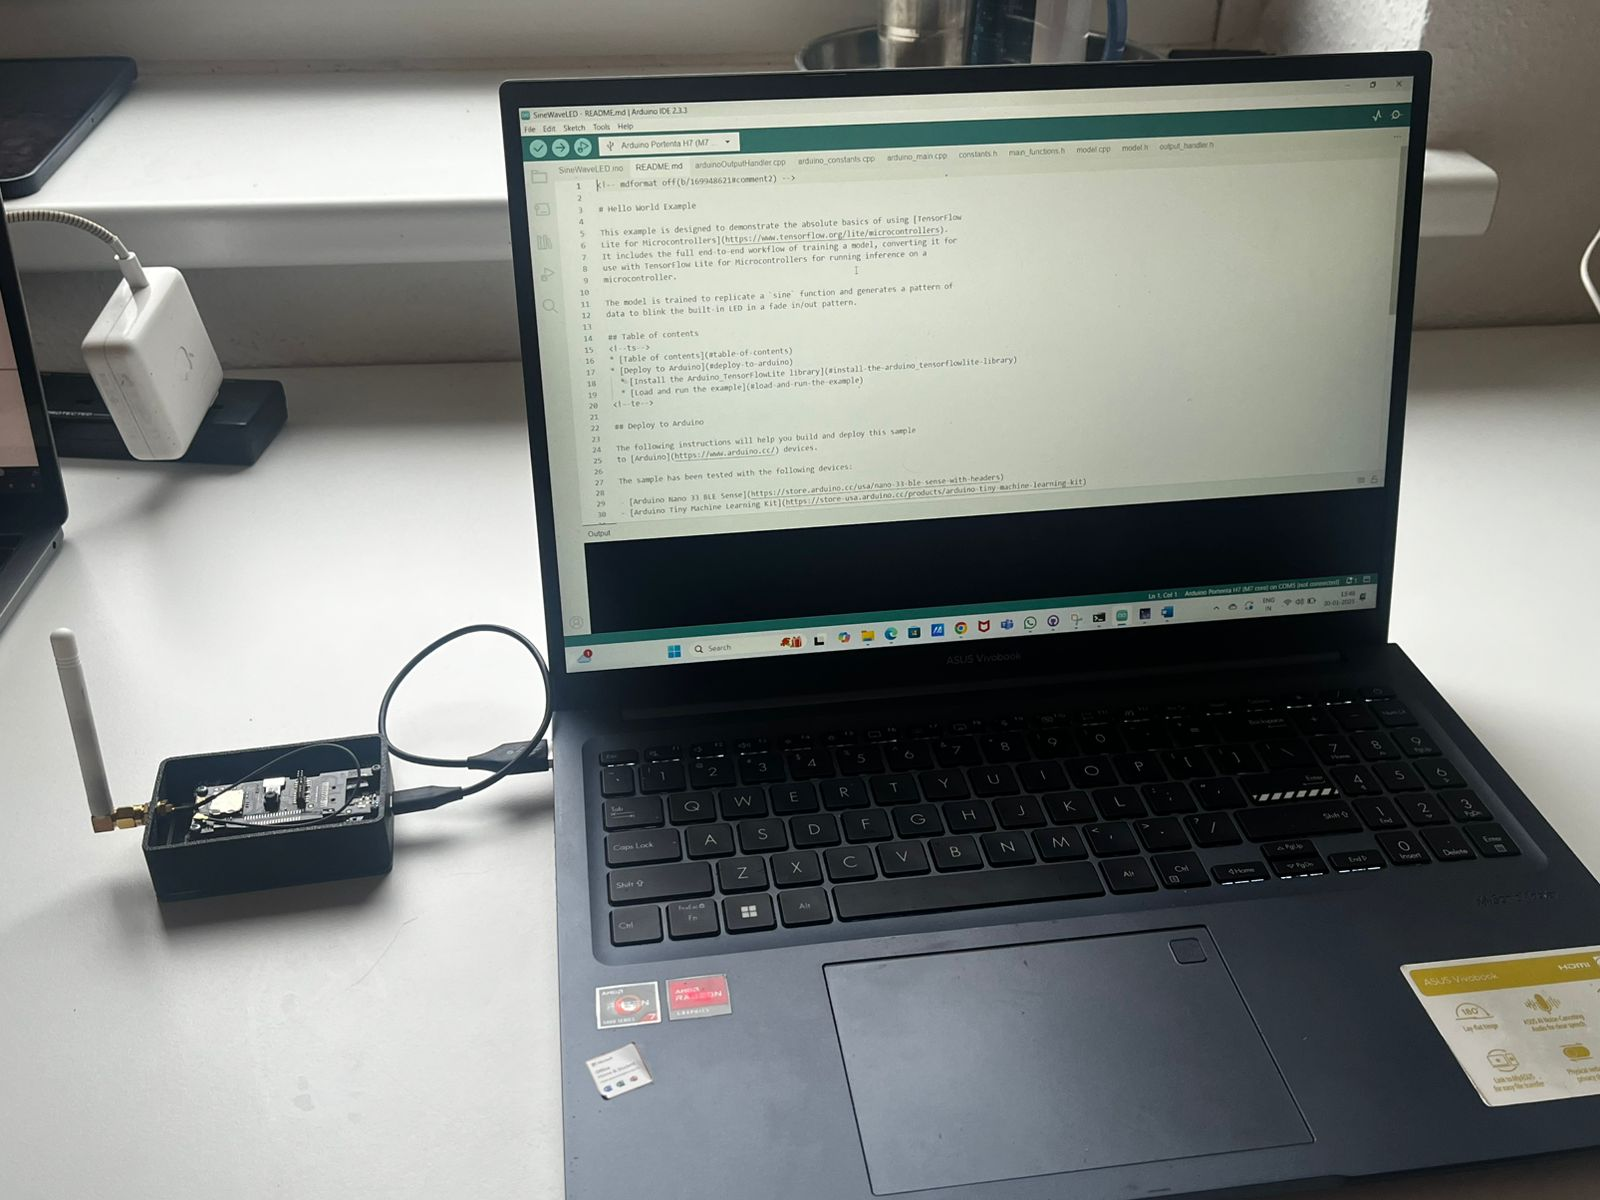
\includegraphics[width=0.7\linewidth]{Images/LORA/LORA2.jpg}
		\caption{LoRa with Antenna}
		\label{LoRAWANRange} 
	\end{center}
\end{figure}

\begin{itemize}
	\item \textbf{Function:} Facilitates the transmission and reception of LoRa signals \cite{semtech_lora:2025}.
	\item \textbf{Antenna Type:} External antenna connected via a \textbf{U.FL connector}, designed to enhance signal quality and maintain a stable communication range \cite{murata_transceiver:2025}.
	\item \textbf{Considerations:} Optimized for compatibility with LoRa frequency bands and to maximize the communication range in different environments \cite{semtech_lora:2025}.
\end{itemize}

\subsection{Microcontroller Unit (MCU)}
\begin{itemize}
	\item \textbf{Function:} Serves as the control center for LoRa operations, handling data processing, interfacing with the transceiver, and managing communication protocols \cite{arduino_portenta:2025}.
	\item \textbf{MCU in Portenta H7:} 
	\begin{enumerate}
		\item Dual-core architecture: ARM Cortex-M7 (480 MHz) for high-performance tasks and Cortex-M4 (240 MHz) for low-power operations 
		\item Ensures efficient management of LoRa-specific operations like encoding/decoding packets and power optimization.\cite{arm_cortex:2025}
	\end{enumerate}
\end{itemize}

\subsection{Power Supply}
\begin{itemize}
	\item \textbf{Function:} Supplies power to the LoRa transceiver and its supporting components 
	\item \textbf{Sources:} The Vision Shield relies on the Portenta H7’s onboard power supply and is compatible with external battery packs for portable LoRa applications 
	\item \textbf{Components:} Includes voltage regulators and power management ICs to ensure stable operation of the LoRa transceiver and optimize battery life during transmission \cite{arduino_portenta:2025}.
\end{itemize}

\subsection{Interface}
\begin{itemize}
	\item \textbf{Function:} The LoRa transceiver communicates with the Portenta H7 via different protocols, which ensures fast and reliable data transfer between the MCU and the LoRa module.
	\item \textbf{Configuration:} Communicates with the MCU using I2C, SPI, or UART protocols \cite{arduino_portenta:2025}.
\end{itemize}

\subsection{Memory}
\begin{itemize}
	\item \textbf{Function:} Provides storage for firmware, LoRa communication logs, and configuration data.
	\item \textbf{Memory in Portenta H7:} 
	\begin{enumerate}
		\item \textbf{Flash Memory:} 16 MB NOR Flash for storing LoRa firmware and application-specific code.
		\item \textbf{SRAM:} 8 MB SDRAM for temporary data processing during LoRa communication \cite{arduino_portenta:2025}.
	\end{enumerate}
\end{itemize}


\begin{table}[h!]
	\centering
	\small % Reduce the font size of the table
	\caption{Specifications of LoRa Device on Portenta Vision Shield} \cite{portenta_lora_specifications:2025}
	\begin{tabular}{|p{4.5cm}|p{8cm}|} % Set fixed column widths
		\hline
		\textbf{Parameter}             & \textbf{Description}                                  \\ \hline
		Module Size                    & Compact, integrated into the Vision Shield           \\ \hline
		Frequency Range                & 868 MHz / 915 MHz (region-specific frequencies for LoRa communication) \\ \hline
		Modulation                     & Long Range (LoRa) modulation and Frequency-Shift Keying (FSK) \\ \hline
		Data Rate                      & 0.3 kilobits per second to 50 kilobits per second    \\ \hline
		Communication Range            & Up to 10 kilometers in open areas with line of sight \\ \hline
		Interface                      & Supports communication with microcontrollers through SPI \\ \hline
		Operating Voltage              & Operates at a typical voltage of 3.3 volts          \\ \hline
		Power Output                   & Output power up to +22 decibel-milliwatts (dBm) \\ \hline
		Operating Temperature          & Functional within a range of -20°C to +70°C         \\ \hline
		Power Consumption (Transmit)   & 20 to 120 milliamperes, depending on the transmission power \\ \hline
		Power Consumption (Receive)    & 10 to 15 milliamperes during reception              \\ \hline
		Sleep Mode Current             & Less than 1 microampere in sleep mode               \\ \hline
		Antenna Connector              & Uses a U.FL connector, a small and reliable connector for attaching an external antenna \\ \hline
	\end{tabular}
	\label{tab:general-specifications} 
\end{table}


\subsection{Peer-To-Peer (P2P) LoRa Communication}
To understand the unique value proposition of LoRaWAN P2P Communication, we first have to understand the network architecture of LoRaWAN(Refer figure ~\ref{TTN1}), which consists of four major components: \cite{SeeedP2PLoRa2021}

\begin{enumerate}
	\item \textbf{End Nodes:} Represents edge devices or sensors
	\item \textbf{Gateway:} Collects or concentrates data from several end nodes
	\item \textbf{Network Server:} Consolidates data from gateways for upload to application server
	\item \textbf{Application Server:} Processes or displays consolidated data \cite{SeeedP2PLoRa2021}
\end{enumerate}

\begin{figure}
	\begin{center}
		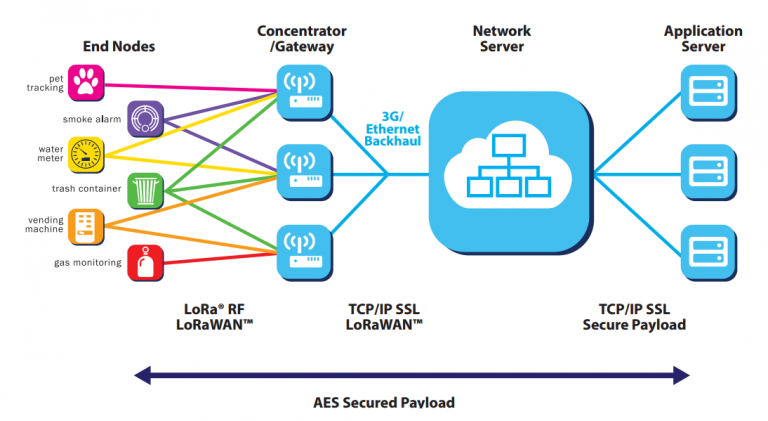
\includegraphics[width=0.7\linewidth]{Images/LORA/TTN1.png}
		\caption{Source: The Things Network}
		\label{TTN1} 
	\end{center}
\end{figure}

End nodes contain sensors that collect valuable information to be transmitted to the cloud. This is done by broadcasting LR data packets to nearby LoRaWAN gateways, which then forward the data to the cloud. Since all gateways in range of the transmitting end node receive the data, this creates a star-on-star topology which promotes dense interconnectivity and reliability in LoRaWAN networks, shown below: 

\begin{figure}
	\begin{center}
		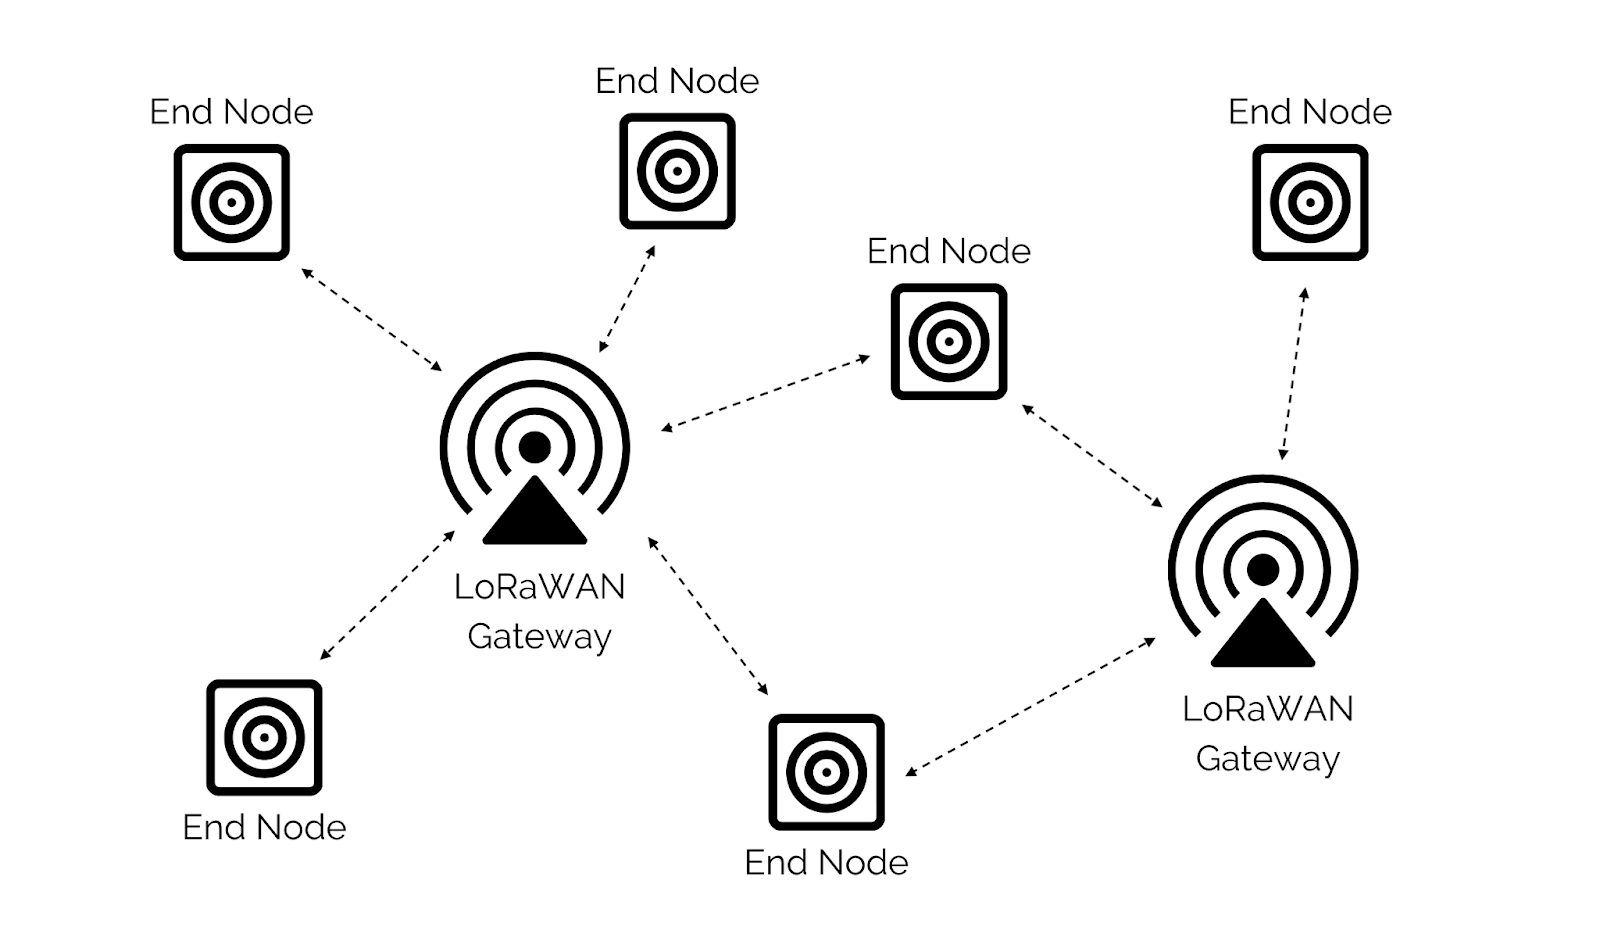
\includegraphics[width=0.7\linewidth]{Images/LORA/LoRaWAN Topology.png}
		\caption{LoRaWAN Topology}
		\label{LoRaWAN Topology} \cite{SeeedP2PLoRa2021}
	\end{center}
\end{figure}

\SHELL{P2P LR Communication} refers to LR communications that occur directly between end node devices (peer-to-peer), instead of those that occur between an end node and the gateway. This communication uses the same long-distance LR modulation between the two devices, and enables numerous possibilities with LR technology! \cite{SeeedP2PLoRa2021}

\begin{figure}
	\begin{center}
		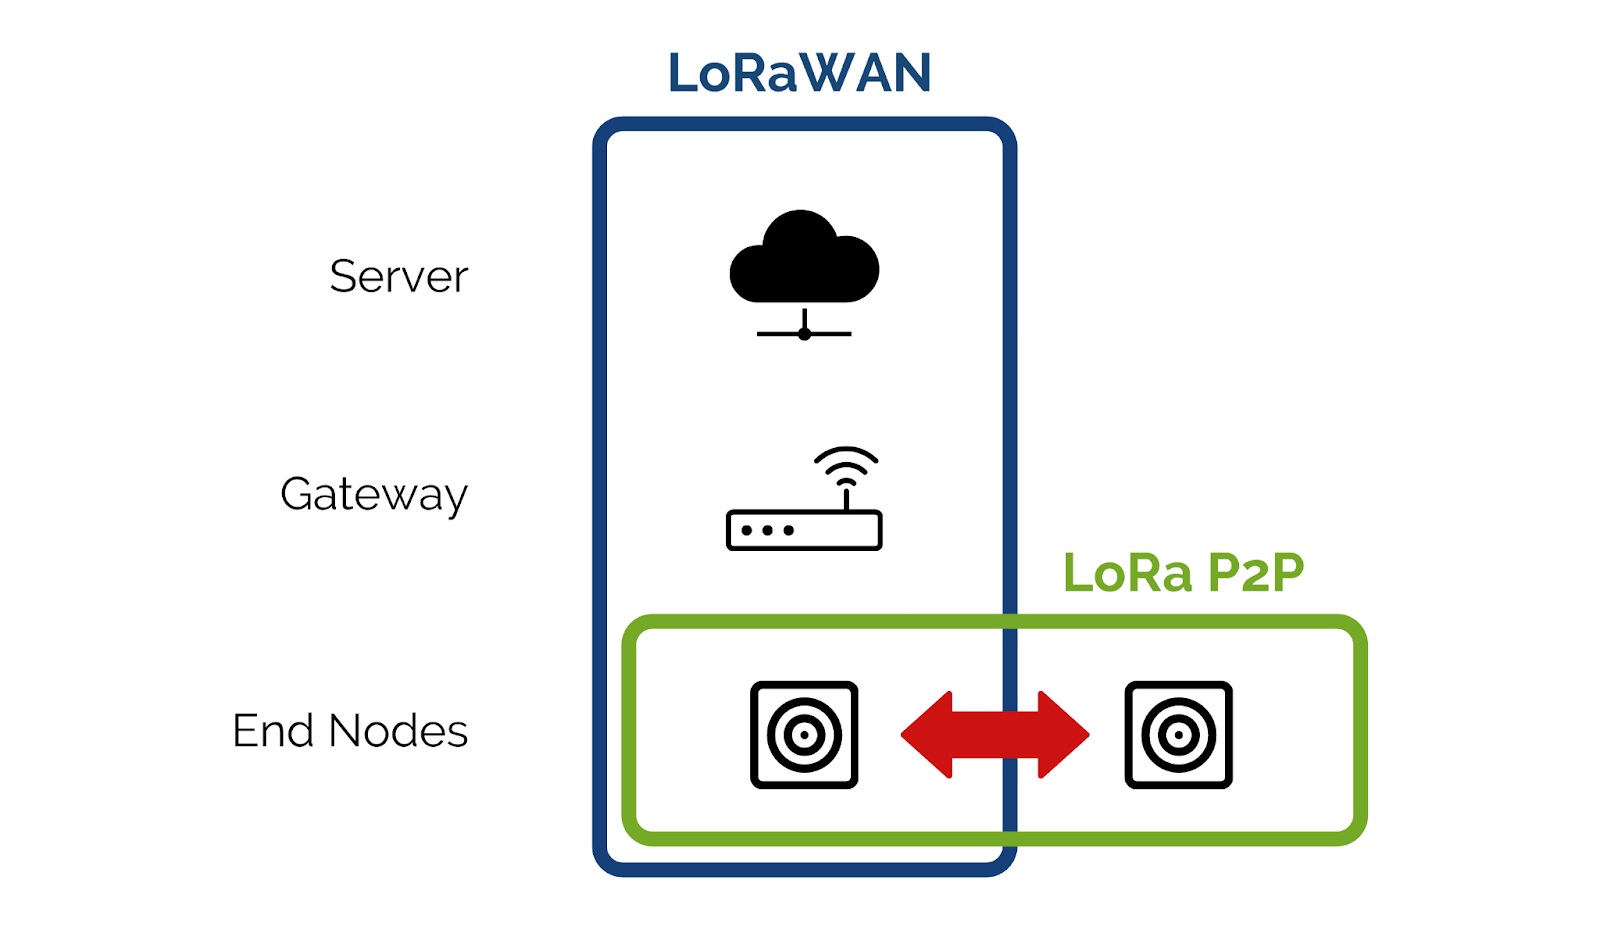
\includegraphics[width=0.7\linewidth]{Images/LORA/P2P LoRa.png}
		\caption{P2P LoRa}
		\label{P2P LoRa} \cite{SeeedP2PLoRa2021}
	\end{center}
\end{figure}

\subsubsection{Benefits of P2P LoRa Communication}

The design of the LoRaWAN network architecture has its own purpose and benefits, which we’ve discussed in depth here. Nonetheless, P2P in LoRaWAN allows end nodes to communicate directly without the use of a gateway, which brings several benefits. \cite{SeeedP2PLoRa2021}

\begin{itemize}
	\item \textbf{Increase the Range of LoRaWAN Coverage} 
	In some areas, the full LoRaWAN infrastructure may be unavailable or unfeasible to set up. By linking multiple end nodes together, we can create a \SHELL{chain topology} that extends the range of the LoRaWAN with a limited additional cost!
	\item \textbf{Reduce Costs of Using LR for IoT}
	Although LoRaWAN gateways are relatively affordable, small-scale applications may benefit from bypassing the use of an additional device to save further costs. This is a great advantage for beginners who are just getting started and want to simply experiment with LoRa.
	\item \textbf{Increased Flexibility with LoRaWAN Networks}
	Did you know that end nodes engaged in P2P LR communication can continue to interface with nearby LoRaWAN Gateways? When used together, P2P connections can be used to further reinforce the LoRaWAN network, providing greater operational reliability. \cite{SeeedP2PLoRa2021}
\end{itemize}

For detailed explanation, please refer the following example ~\ref{P2P}.



\section{Low-Power Wide Area Networks(LPWAN)} 

Low-Power Wide Area Networks (LPWAN) is a group of wireless networks technologies well suited to the specific needs of IoT devices: low-bandwidth and low-power devices, usually battery-powered. This type of networks provide low-bit rates long ranges with a low-power consumption. LPWAN's can accommodate data packets sizes from 10 bytes to 1 kB at uplink speeds up to 200 kbps; long-range connectivity varies from 2 to 1,000 km depending on the network technology. Most LPWAN's technologies have a star topology; this means that each device connects directly to a central access point. \cite{ArduinoLoRaWAN101:2024}

Some of the important use cases for LPWAN's include the following applications:

\begin{enumerate}
	\item \textbf{Smart cities:} smart parking, intelligent street lighting.
	\item \textbf{Supply chain management:} asset tracking, condition monitoring.
	\item \textbf{Smart grids:} electricity, water, and gas metering.
	\item \textbf{Smart agriculture:} land condition monitoring, animal tracking, geofencing. \cite{ArduinoLoRaWAN101:2024}
\end{enumerate}

Several LPWAN technologies use licensed or unlicensed frequencies and proprietary or open specifications. LoRa and its Media Access Control (MAC) layer protocol implementation, LoRaWAN, is currently one of the existing LPWAN gaining the most traction to support IoT devices and services. 


\subsection{Difference between LoRa and LoRaWAN?} 
LoRa is a wireless modulation technique derived from Chirp Spread Spectrum (CSS) technology. CSS uses wideband linear frequency modulated chirp pulses to encode information. LoRa can operate on the following license-free sub-gigahertz ISM (Industrial, Scientific, and Medical) bands: 433 MHz, 868 MHz, and 915 MHz. ISM bands are internationally reserved for industrial, scientific and, medical uses. 
\newline

Based on LoRa, the LoRaWAN (LoRa for Wide Area Networks) specification extended the LoRa physical communication layer into the Internet by adding a MAC layer(Refer Figure ~\ref{NetworkLayer}). The LoRaWAN specification is a software layer that defines how devices must use the LoRa, for example, when they transmit or receive messages. The LoRaWAN specification is open-source; it has been supported and maintained by the LoRa Alliance since 2015. \cite{ArduinoLoRaWAN101:2024}

\subsection{LoRaWAN Network Architecture}

A typical LoRaWAN network architecture includes the following essential parts: end-devices (usually sensors), a base station or gateway, also known as Long Range Relay (LRR), a network server also known as Long Range Controller (LRC), and the Operation Support System (OSS) for provisioning and management of the network.
\cite{ArduinoLoRaWAN101:2024}

\begin{figure}
	\begin{center}
		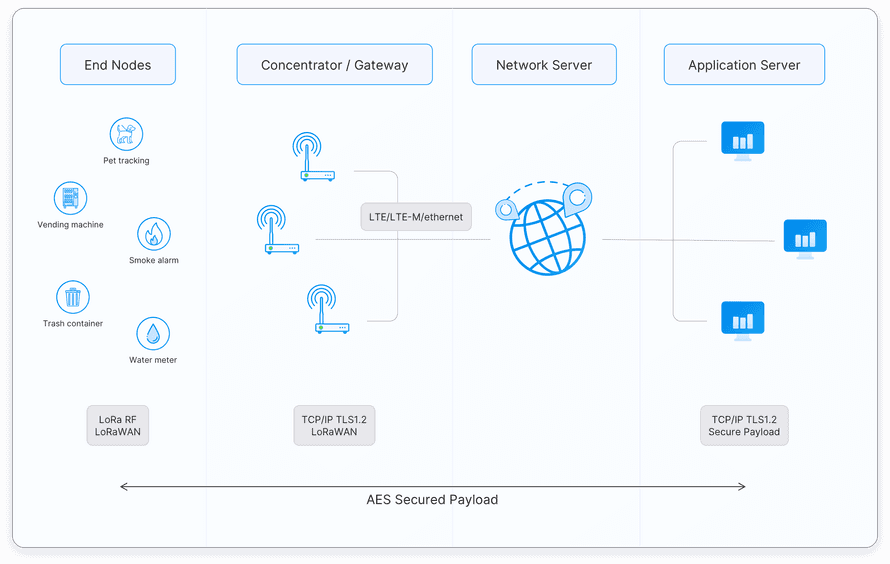
\includegraphics[width=0.7\linewidth]{Images/LORA/LoRaWANArch.png}
		\caption{Typical LoRaWAN network architecture example.}
		\label{LoRaWANArch} 
	\end{center}
\end{figure}

Refer image ~\ref{LoRaWANArch}, notice there is a fundamental difference between a network server and a gateway. The network server controls the virtualized MAC layer of the LoRaWAN network while gateways are devices pre-integrated with the network server to ease the LPWAN rollout and provisioning. LoRaWAN network servers and gateways access can be public or private. 

LoRaWAN networks are usually deployed in a star-of-stars topology; this means that gateways manage data between end-devices and a network server. Gateways are connected to the central network server via the Internet, while end-devices use LoRa to send and receive data to and from the gateways; end-devices are not exclusively tied to a single gateway, end-devices broadcast information to all the gateways in range. Communication in LoRaWAN networks is natively bi-directional, although uplink communication between end-devices and the central network server is expected to be predominant in the network. \cite{ArduinoLoRaWAN101:2024}

Star networks present several advantages compared to other network topologies:

\begin{itemize}
	\item Gateways can be added to the network anywhere and anytime without prior planning.
	\item Message delivery is more robust since multiple gateways receive the same data packets during each uplink. \cite{ArduinoLoRaWAN101:2024}
\end{itemize}

\subsection{Data Rates}

Communication between end-devices and gateways in LoRaWAN networks is spread out on different frequency channels and data rates (communications using different data rates do not interfere with each other).

\textbf{LoRa supports data rates ranging from 300 bps to 5 kbps for a 125 kHz bandwidth.}
\newline

To maximize the battery life of each end-device and the overall capacity available through the network, LoRaWAN uses an Adaptive Data Rate (ADR) mechanism for optimizing data rates, airtime, and power consumption. ADR controls the following transmission parameters on end-devices: \cite{ArduinoLoRaWAN101:2024}

\begin{enumerate}
	\item \textbf{Spreading factor:} the speed of data transmission. Lower spreading factors mean a higher data transmission rate.
	\item \textbf{Bandwidth:}the amount of data that can be transmitted from one point to another within the network.
	\item \textbf{Transmission power:}the energy that the end-device transmitter produces at its output. \cite{ArduinoLoRaWAN101:2024}
\end{enumerate}

The table below ~\ref{tab:spreading-factor-specifications} shows compares spreading factor, data rate, and time on-air at a bandwidth of 125 kHz (range is an indicative value, it will depend on the propagation conditions):

\begin{table}[h!]
	\centering
	\caption{LoRa Spreading Factor Specifications} 
	\begin{tabular}{|l|l|l|l|}
		\hline
		\textbf{Spreading Factor (SF)} & \textbf{Data Rate (bps)} & \textbf{Range (km)} & \textbf{Time on-Air (ms)} \\ \hline
		SF7                            & 5470                    & 2                   & 56                       \\ \hline
		SF8                            & 3125                    & 4                   & 100                      \\ \hline
		SF9                            & 1760                    & 6                   & 200                      \\ \hline
		SF10                           & 980                     & 8                   & 370                      \\ \hline
		SF11                           & 440                     & 11                  & 40                       \\ \hline
		SF12                           & 290                     & 14                  & 1400                     \\ \hline
	\end{tabular}
	\label{tab:spreading-factor-specifications} 
\end{table}

End-devices may transmit on any channel available at any time, using any available data rate, as long as the following rule is respected:

\begin{itemize}
	\item The end-device changes channel in a pseudo-random fashion for every transmission. The resulting frequency diversity makes the system more robust against interference. \cite{ArduinoLoRaWAN101:2024}
\end{itemize}

Also, local regulations must be respected, for example:

\begin{itemize}
	\item In the EU868 band, the end-device must respect the maximum transmit duty cycle relative to the sub-band used and local regulations (1% for end-devices).
	\item In the US915 band, the end-device must respect the maximum transmit duration (or dwell time) relative to the sub-band used and local regulations (400ms). \cite{ArduinoLoRaWAN101:2024}
\end{itemize}

\begin{figure}
	\begin{center}
		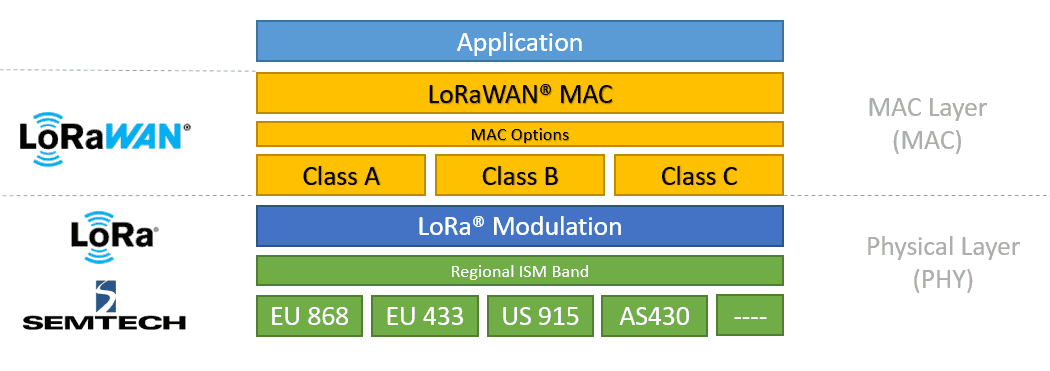
\includegraphics[width=0.7\linewidth]{Images/LORA/NetworkLayer.png}
		\caption{LoRaWAN network layers. Image credits: Semtech.}
		\label{NetworkLayer} 
	\end{center}
\end{figure}

\subsection{Classes}

The LoRaWAN specification has three different communication profiles between devices and applications: \SHELL{Class A, Class B, and Class C.} (Refer figure ~\ref{NetworkLayer}) Each class serves different application needs and has optimized requirements for specific purposes. The main difference between the three classes is latency and power consumption; end-devices can always send uplinks when needed, but its class will determine when to receive downlinks. \cite{ArduinoLoRaWAN101:2024}

\subsubsection{Class A: "Aloha"}

Class A devices implement a bi-directional communication profile where two short downlinks follow the end-device uplink transmission receive windows, usually referred to as RX1 and RX2. If the server does not respond in either RX1 or RX2 windows, the next opportunity will be after the next uplink transmission(Refer figure ~\ref{ClassAProfile}). Class A devices are often battery-powered and spend most of the time in sleep mode; therefore, they have the lowest energy consumption, keep long intervals between uplinks, and have high downlink latency.  \cite{ArduinoLoRaWAN101:2024}

\begin{figure}
	\begin{center}
		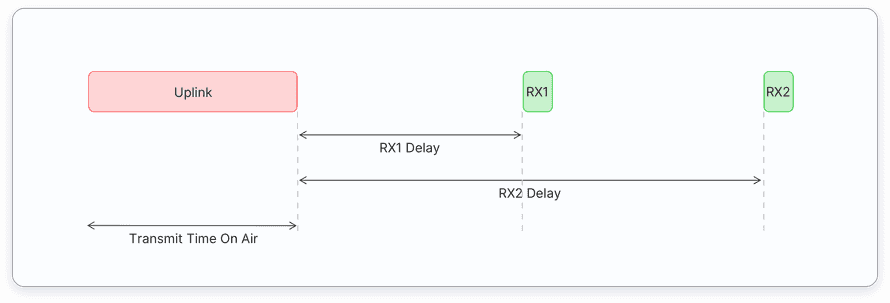
\includegraphics[width=0.7\linewidth]{Images/LORA/ClassAProfile.png}
		\caption{Class A default configuration profile. Image credits: The Things Network.}
		\label{ClassAProfile} 
	\end{center}
\end{figure}

\subsubsection{Class B: The "Beaconing" Class}

Class B devices extend Class A devices by adding scheduled receive windows for downlinks, and, therefore, they emulate a continuously receiving device by opening receive windows at fixed time intervals(Refer figure ~\ref{ClassBProfile}). This class should be implemented when low latency of downlink communication while keeping the power consumption as low as possible is required.  \cite{ArduinoLoRaWAN101:2024}

\begin{figure}
	\begin{center}
		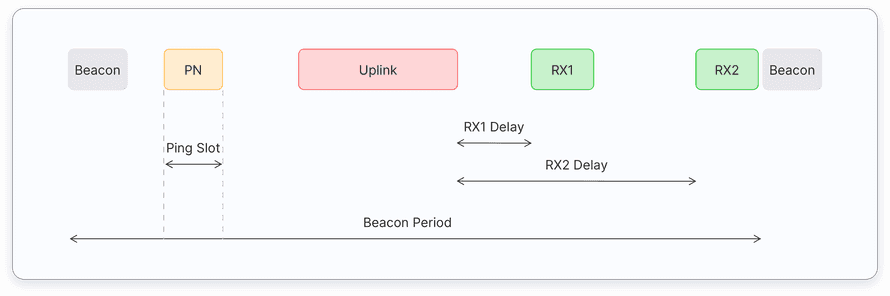
\includegraphics[width=0.7\linewidth]{Images/LORA/ClassBProfile.png}
		\caption{Class B default configuration profile. Image credits: The Things Network.}
		\label{ClassBProfile} 
	\end{center}
\end{figure}

\subsubsection{Class C: Continuous Reception}

Class C communication profile is used in applications with enough power available, so there is no need to minimize the time of the reception windows(Refer figure ~\ref{ClassCProfile}); this is the case of most actuators (e.g., smart plugs, street lights, electrical meters, etc.) Class C devices always listen for downlinks messages unless they transmit an uplink message. This behavior results in the lowest latency between the server and the end-device.  \cite{ArduinoLoRaWAN101:2024}

\begin{figure}
	\begin{center}
		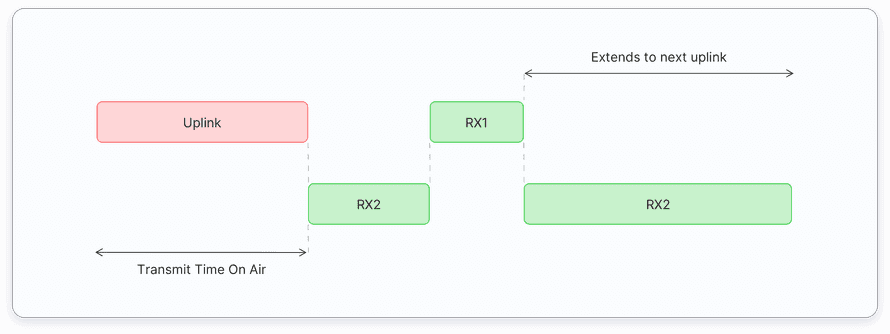
\includegraphics[width=0.7\linewidth]{Images/LORA/ClassCProfile.png}
		\caption{Class C default configuration profile. Image credits: The Things Network}
		\label{ClassCProfile}
	\end{center}
\end{figure}

\subsection{Authentication and Security}

Authentication and security are also important in LoRaWAN networks. Any LoRaWAN network has a baseline authentication and security framework based on the AES 128 encryption scheme. Compared to other LPWAN's, which rely on a single key for authentication and encryption, the LoRaWAN framework separates both. Authentication and integrity control use a network session key (NwkSKey) while user data encryption uses an application session key (AppSKey). \cite{ArduinoLoRaWAN101:2024}

NwkSKey and AppSKey are AES-128 root keys specific to the end-device, end-devices manufacturers, or application owners assigned them.

LoRaWAN supports two authentication and activation methods: Over-The-Air-Activation (OTAA) and Activation by Personalization (ABP).

\begin{enumerate}
	\item \textbf{Over-The-Air Activation (OTAA):} In this method, end-devices are not initialized for any particular network; they send a JOIN request to a specific LoRaWAN network and then receive a device address and an authorization token from which session keys are derived(Refer figure ~\ref{OTAA}); NwkSKey and AppSKey are derived during this procedure from a root AppKey pre-provisioned in the end-devices by its manufacturer. \cite{ArduinoLoRaWAN101:2024} 
	
	\begin{figure}
		\begin{center}
			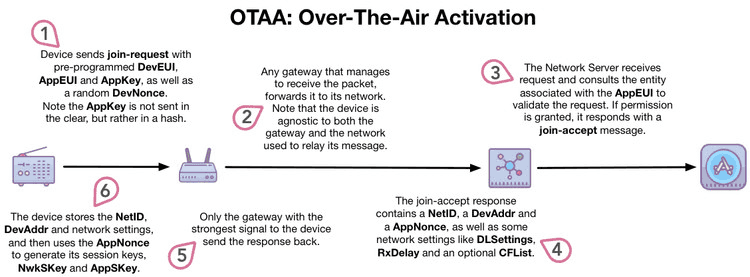
\includegraphics[width=0.7\linewidth]{Images/LORA/OTAA.png}
			\caption{Over-The-Air activation process. Image credits: Heath Raftery.}
			\label{OTAA} 
		\end{center}
	\end{figure}
	
	\item \textbf{Activation by Personalization (ABP):} In this method, end-devices are personalized to work with a given LoRaWAN network. End-devices are pre-provisioned with the NwkSKey and AppSKey and the 32-bits device network address(Refer figure ~\ref{Activation}). \cite{ArduinoLoRaWAN101:2024}
	
	\begin{figure}
		\begin{center}
			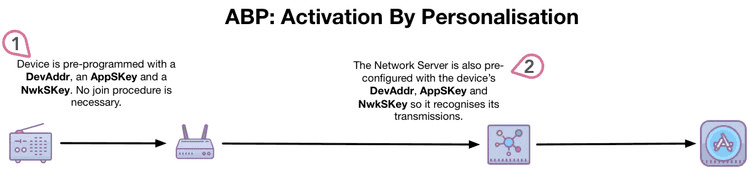
\includegraphics[width=0.7\linewidth]{Images/LORA/Activation.png}
			\caption{Activation by Personalization process. Image credits: Heath Raftery.}
			\label{Activation} 
		\end{center}
	\end{figure}	
	
\end{enumerate}


\subsection{Connecting to the LoRaWAN-TTN}
The Portenta Vision Shield - LoRa can be connected to the TTN and can transmit data to other devices connected to this network through a secure channel. This channel is nothing but an application on the TTN network dedicated for your board. In this tutorial, you will be guided through a step-by-step process of setting up your Portenta board and the Vision Shield - LoRa to communicate with a TTN application. As stated before, to be able to follow this guide, you need to be under coverage of one of the TTN gateways. You can check for the coverage now if you have not done so yet. \cite{ArduinoTTN:2024}
\begin{itemize}
	
	\item \textbf{1. Setting up the Environment} First choose your region. Next, sign in with your The Things Network account(Refer figure ~\ref{Things Network}). If you do not have an account, create a new one on the login page of Things Network. Then fill all the required fields to complete a new registration.
	
	\begin{figure}
		\begin{center}
			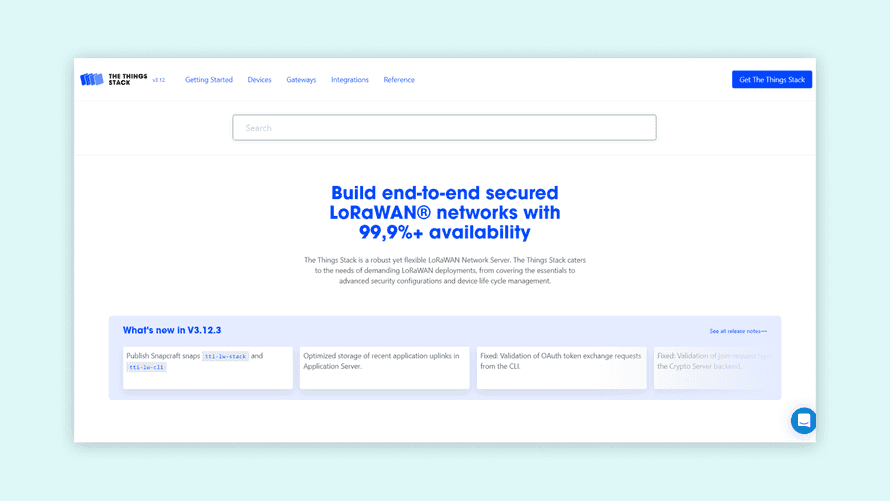
\includegraphics[width=0.7\linewidth]{Images/LORA/ThingsNetwork.png}
			\caption{Things Network}
			\label{Things Network}
		\end{center}
	\end{figure}
	
	\item \textbf{2. Creating an App on TTN} Once you have created an account with TTN, you need to create a TTN application(Refer figure ~\ref{Select Application}). An application provides a way to aggregate data from different devices, and then use these data with other 3rd party integrations. After signing in, click on Create an application, or Go to applications if you already have created one. \cite{ArduinoTTN:2024}
	
	\begin{figure}
		\begin{center}
			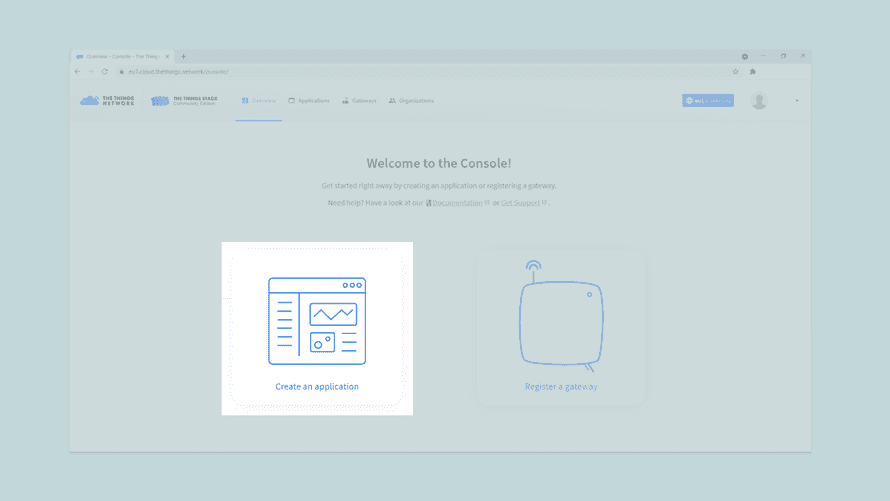
\includegraphics[width=0.7\linewidth]{Images/LORA/SelectApplication.png}
			\caption{Select Application}
			\label{Select Application}
		\end{center}
	\end{figure}
	
	Here you will have a list of all your applications. Now create your first app by pressing the Create an application button.
	
	You have now to fill only the first two fields:
	
	\begin{enumerate}
		\item The first one is the Owner of your app, it will automatically have you as the owner.
		\item The second one is the ID of your app: this must be lowercase and without spaces.
	\end{enumerate}
	
	\begin{figure}
		\begin{center}
			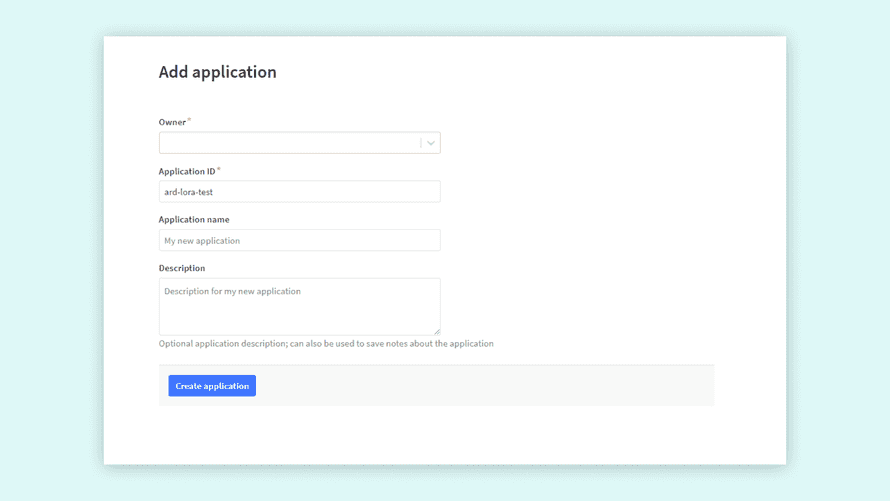
\includegraphics[width=0.7\linewidth]{Images/LORA/AddingApplication.png}
			\caption{AddingApplication}
			\label{AddingApplication} 
		\end{center}
	\end{figure}
	
	After completing these two fields, press the "Create application" button located at the bottom left corner of the page. The dashboard will then show you an overview of the newly created app. \cite{ArduinoTTN:2024}
	
	\begin{figure}
		\begin{center}
			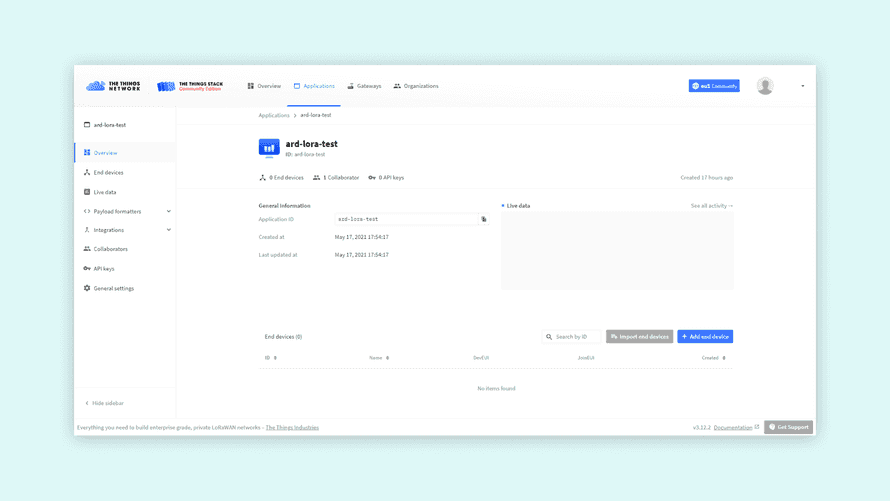
\includegraphics[width=0.7\linewidth]{Images/LORA/AppParameter.png}
			\caption{AppParameter}
			\label{AppParameter} 
		\end{center}
	\end{figure}
	
	Let's take a closer look at these sections:
	\begin{enumerate}
		\item \textbf{Application Overview:} in order to use this app, you will need the Application ID and a device specific AppKey. An EUI is a globally unique identifier for networks, gateways applications and devices. The EUIs are used to identify all parts of the LoRaWAN inside the backend server.
		\item \textbf{End devices:}here you can see and manage all the associated devices (e.g. your Portenta H7 with Portenta Vision Shield - LoRa, Arduino MKR WAN 1300 or MKR WAN 1310), or proceed with the registration of a new one. Registering a new device lets you generate an AppEUI and an AppKey.
		\item \textbf{Collaborators:} here you can see and manage all the app collaborators, to integrate with other collaborative platforms or to manage access rights to the app with other TTN registered profiles.
		\item \textbf{API keys:} here you can create an API key, it is the most sensible information. It is basically the key to gain access to your app, so keep it safe. \cite{ArduinoTTN:2024}
	\end{enumerate}
	
	\item \textbf{3. Configuring the Portenta Vision Shield} It iss now time to connect your Portenta H7 and Portenta Vision Shield - LoRa to TTN. You will need to upload code to the board, so, as you probably already know, there are two options:
	
	Use the Arduino Cloud Editor
	
	Use the Arduino IDE, (this is the option this guide will follow)
	
	Plug the Portenta Vision Shield - LoRa to the Portenta H7 and them to your PC through the USB port. Be sure to have selected the right board "Arduino Portenta H7 (M7 core)" and the right port.(Refer figure ~\ref{MCore}) \cite{ArduinoTTN:2024}
	
	\begin{figure}
		\begin{center}
			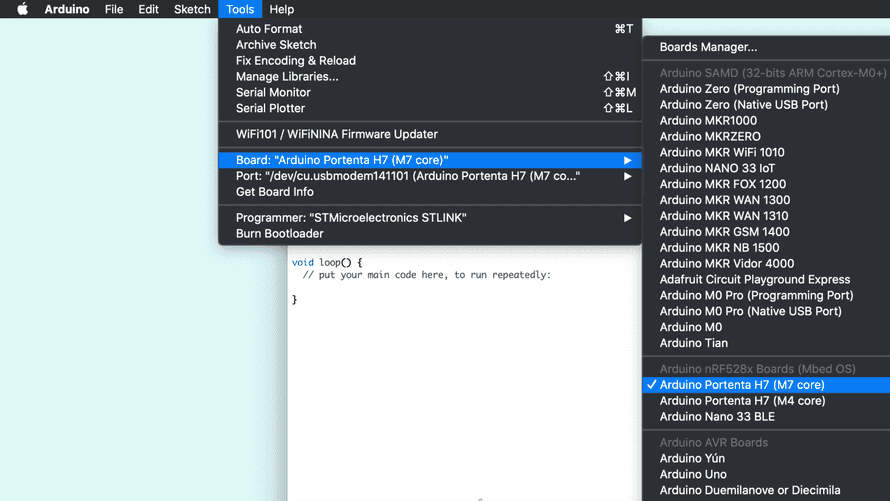
\includegraphics[width=0.7\linewidth]{Images/LORA/MCore.png}
			\caption{MCore}
			\label{MCore}
		\end{center}
	\end{figure}
	
	The LoRa module on the Portenta Vision Shield - LoRa can be accessed by using the \SHELL{MKRWAN library}(if you cannot find it in your examples list, you can go to \SHELL{Tools > Library Manager} and type "MKRWAN library" to install it). This library provides all the APIS to communicate with LoRa and LoRaWAN networks and can be installed from the library Manager. The first code you need to upload and run is from the \SHELL{MKRWAN} library, and its name is \SHELL{FirstConfiguration}. 
	
	\begin{figure}
		\begin{center}
			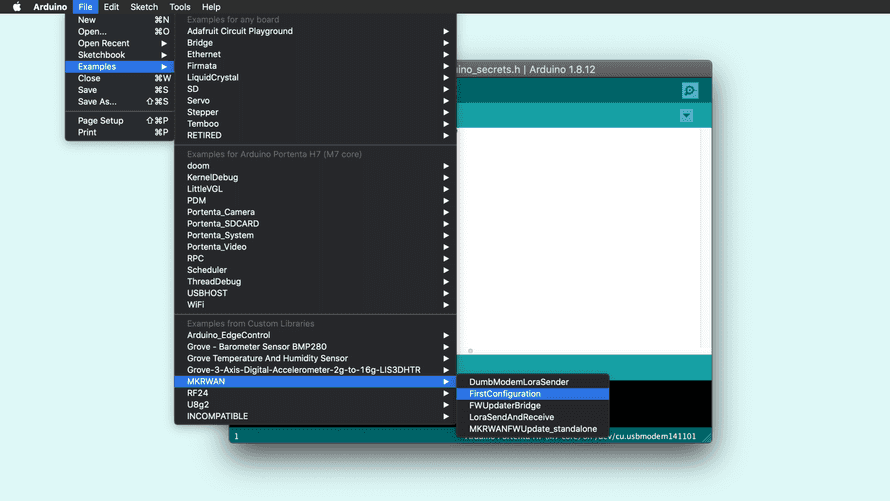
\includegraphics[width=0.7\linewidth]{Images/LORA/UploadCode.png}
			\caption{UploadCode}
			\label{UploadCode} \cite{ArduinoTTN:2024}
		\end{center}
	\end{figure}
	
	The only line you may need to change before uploading the code is the one that sets the frequency. Set the frequency code according to your country if needed. You can find more information about frequency by country at this TTN link.
	
	\begin{lstlisting}[language=C++, frame=single, numbers=left, basicstyle=\ttfamily\small]
		// change this to your regional band (eg. US915, AS923, ...)
		if (!modem.begin(EU868)) {    ...
		\end{lstlisting}
		
		Once you have added to the sketch the frequency according to your country, you can upload it to the board. Then, when the upload is completed, open the Serial Monitor. The following details will show up:
		
		\begin{lstlisting}[language=C++, frame=single, numbers=left, basicstyle=\ttfamily\small]
			Your module version is: ARD-078 1.2.1
			Your device EUI is: a8xxxxxxxxxxxxxx
			Are you connecting via OTAA (1) or ABP (2)?
		\end{lstlisting}
		
		In order to select the way in which the board is going to connect with TTN (OTAA or ABP), you need to configure it on the TTN portal. You will see which option you should select in the following steps. \cite{ArduinoTTN:2024} 
		
		\item \textbf{4. Registering the Portenta on TTN} Before your Portenta H7 can start communicating with the TTN, you need to register the board with an application(Refer figure ~\ref{RegisteringDevice}). Go back to the TTN portal and scroll to End devices section on your Application dashboard, then click Add end device. \cite{ArduinoTTN:2024} 
		
		\begin{figure}
			\begin{center}
				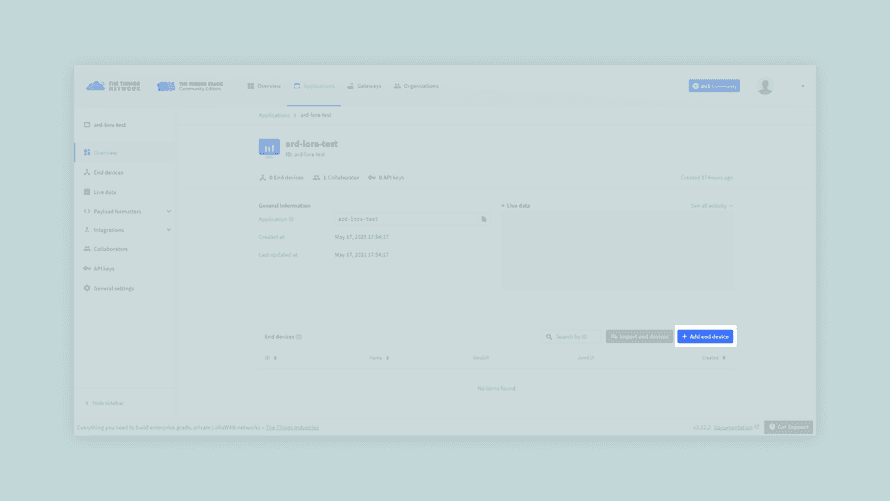
\includegraphics[width=0.7\linewidth]{Images/LORA/RegisteringDevice.png}
				\caption{RegisteringDevice}
				\label{RegisteringDevice} 
			\end{center}
		\end{figure}
		
		On the registration page, first you have to fill in information about your board(Refer figure ~\ref{RegisteringDevice}). Select brand Arduino SA, and Portenta Vision Shield - LoRa as the model. Hardware and firmware versions will automatically be set to the newest ones. Then set your preferred region.
		
		\begin{figure}
			\begin{center}
				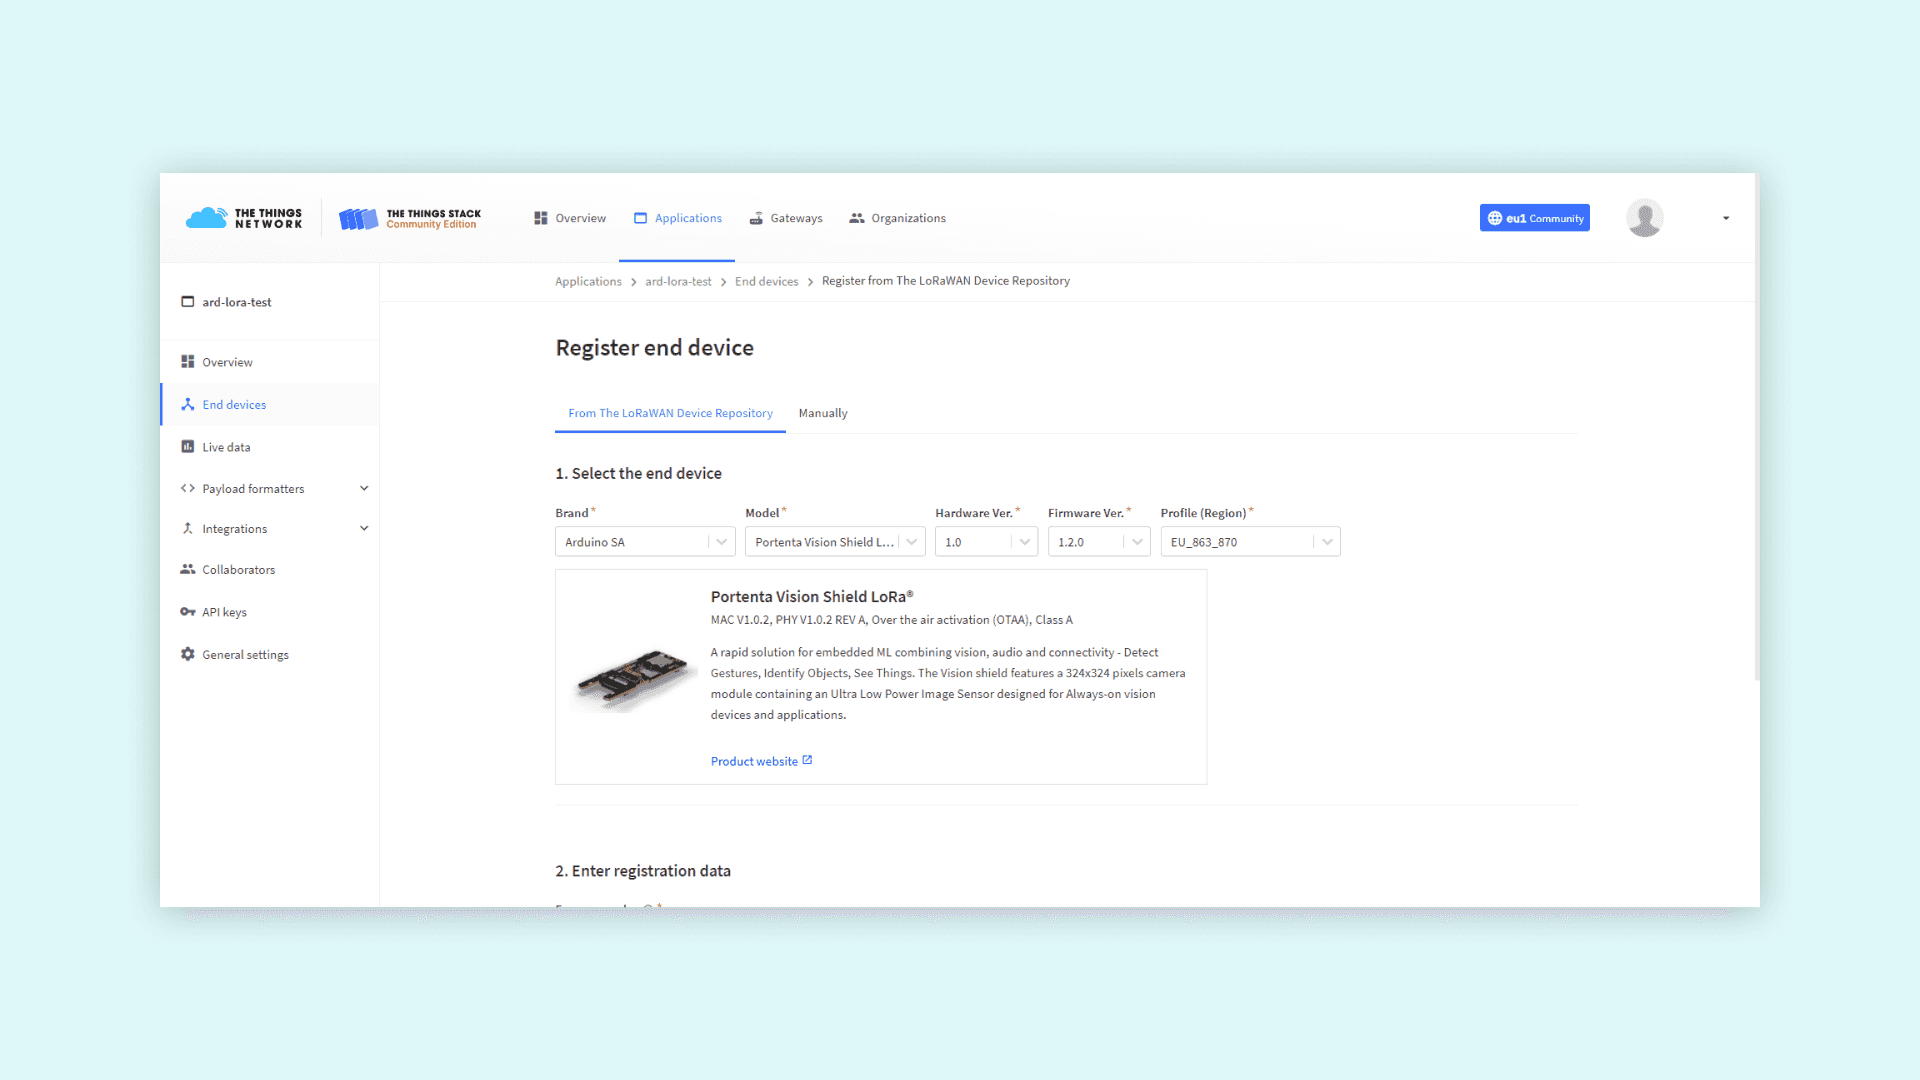
\includegraphics[width=0.7\linewidth]{Images/LORA/DeviceEUI.png}
				\caption{RegisteringDevice}
				\label{RegisteringDevice} 
			\end{center}
		\end{figure}
		
		In the second step of registering the device, fill in End device ID and End device ID(Refer figure ~\ref{Secondstep}). You can click the generate button next to the AppKey field to generate an app key for this device. Similarly, you can press the button next to the AppEUI field to make it all zeros, or enter your own AppEUI.
		
		\SHELL{Note:} The Device ID must be lowercase and without spaces. The \SHELL{DevEUI} should be copied from the Serial Monitor. 
		
		\begin{figure}
			\begin{center}
				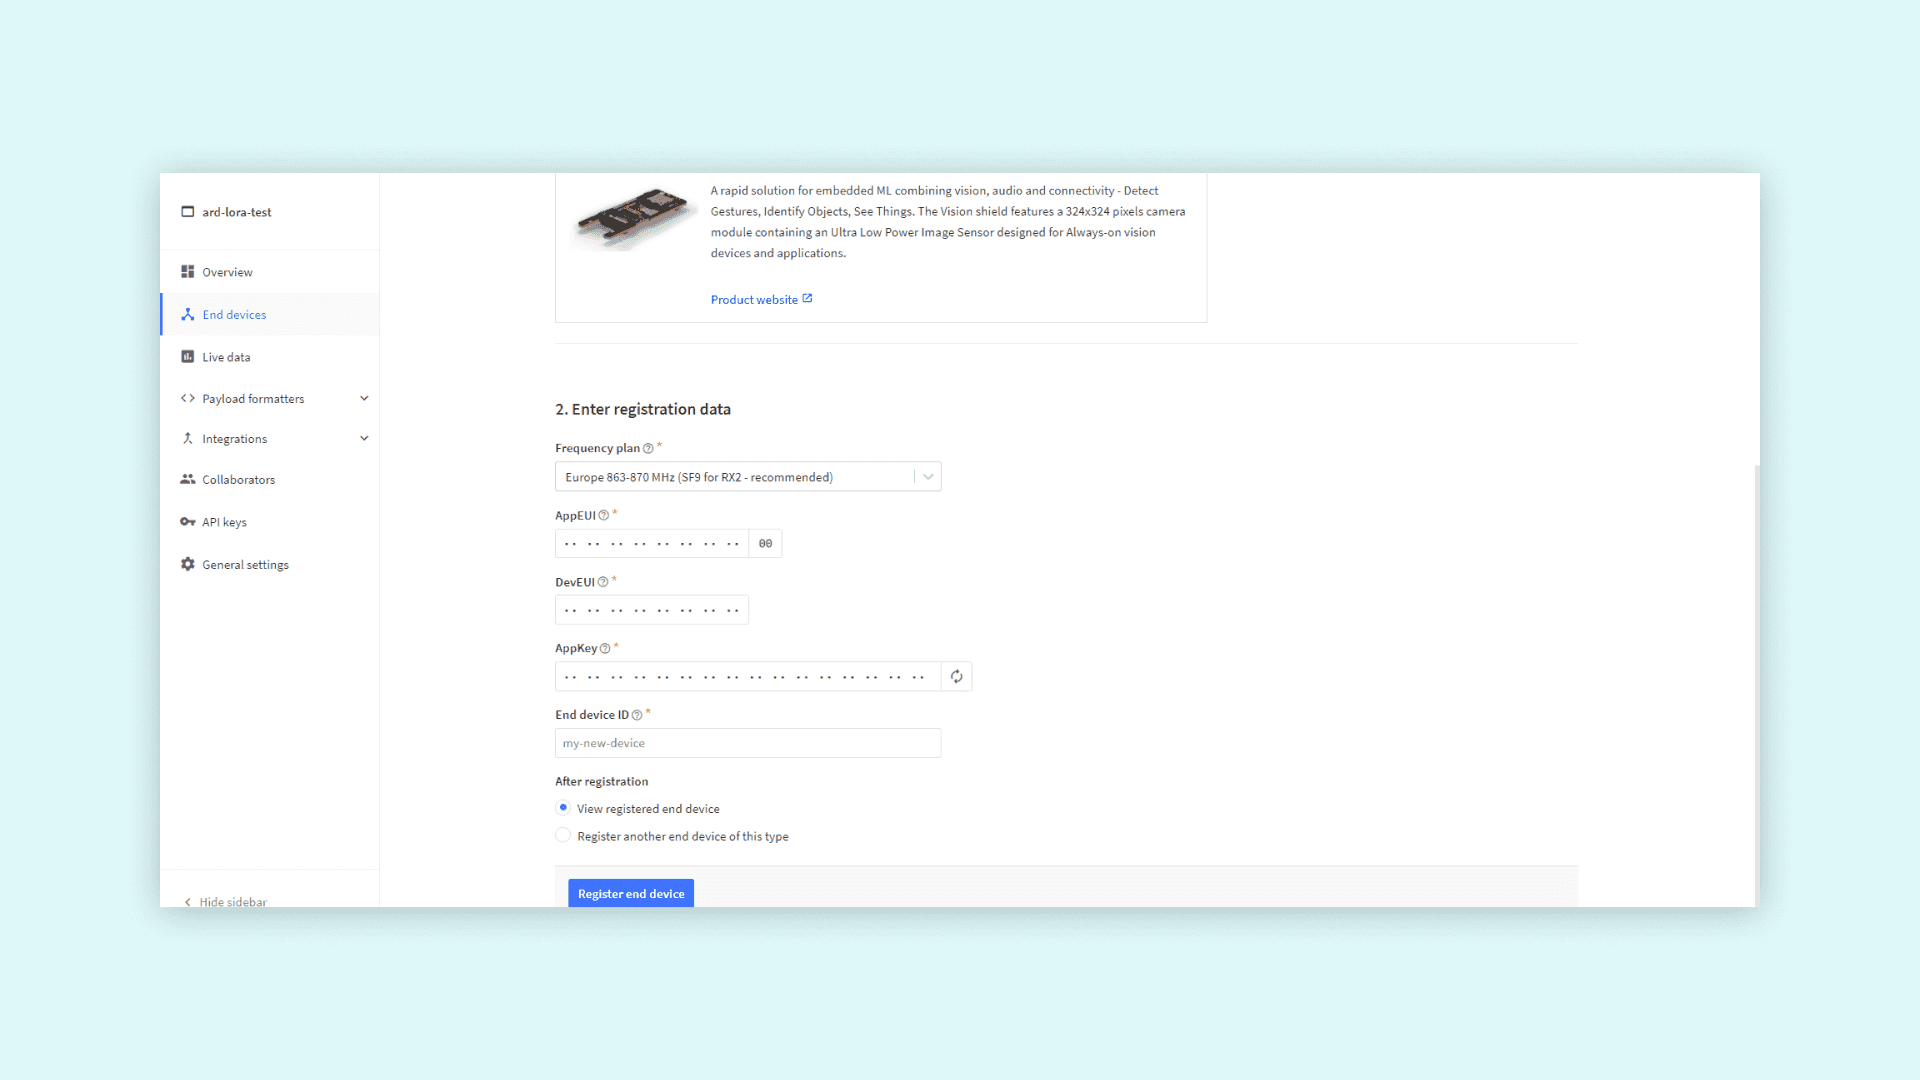
\includegraphics[width=0.7\linewidth]{Images/LORA/Secondstep.png}
				\caption{Secondstep}
				\label{Secondstep} 
			\end{center}
		\end{figure}
		
		After pressing the Register button, your board will show up on the \SHELL{Device Overview} page. You can now see all the information needed to complete the Arduino setup. \cite{ArduinoTTN:2024}
		
		For detailed explanation, please refer the following example ~\ref{LORAWAN}.
		
		\begin{figure}
			\begin{center}
				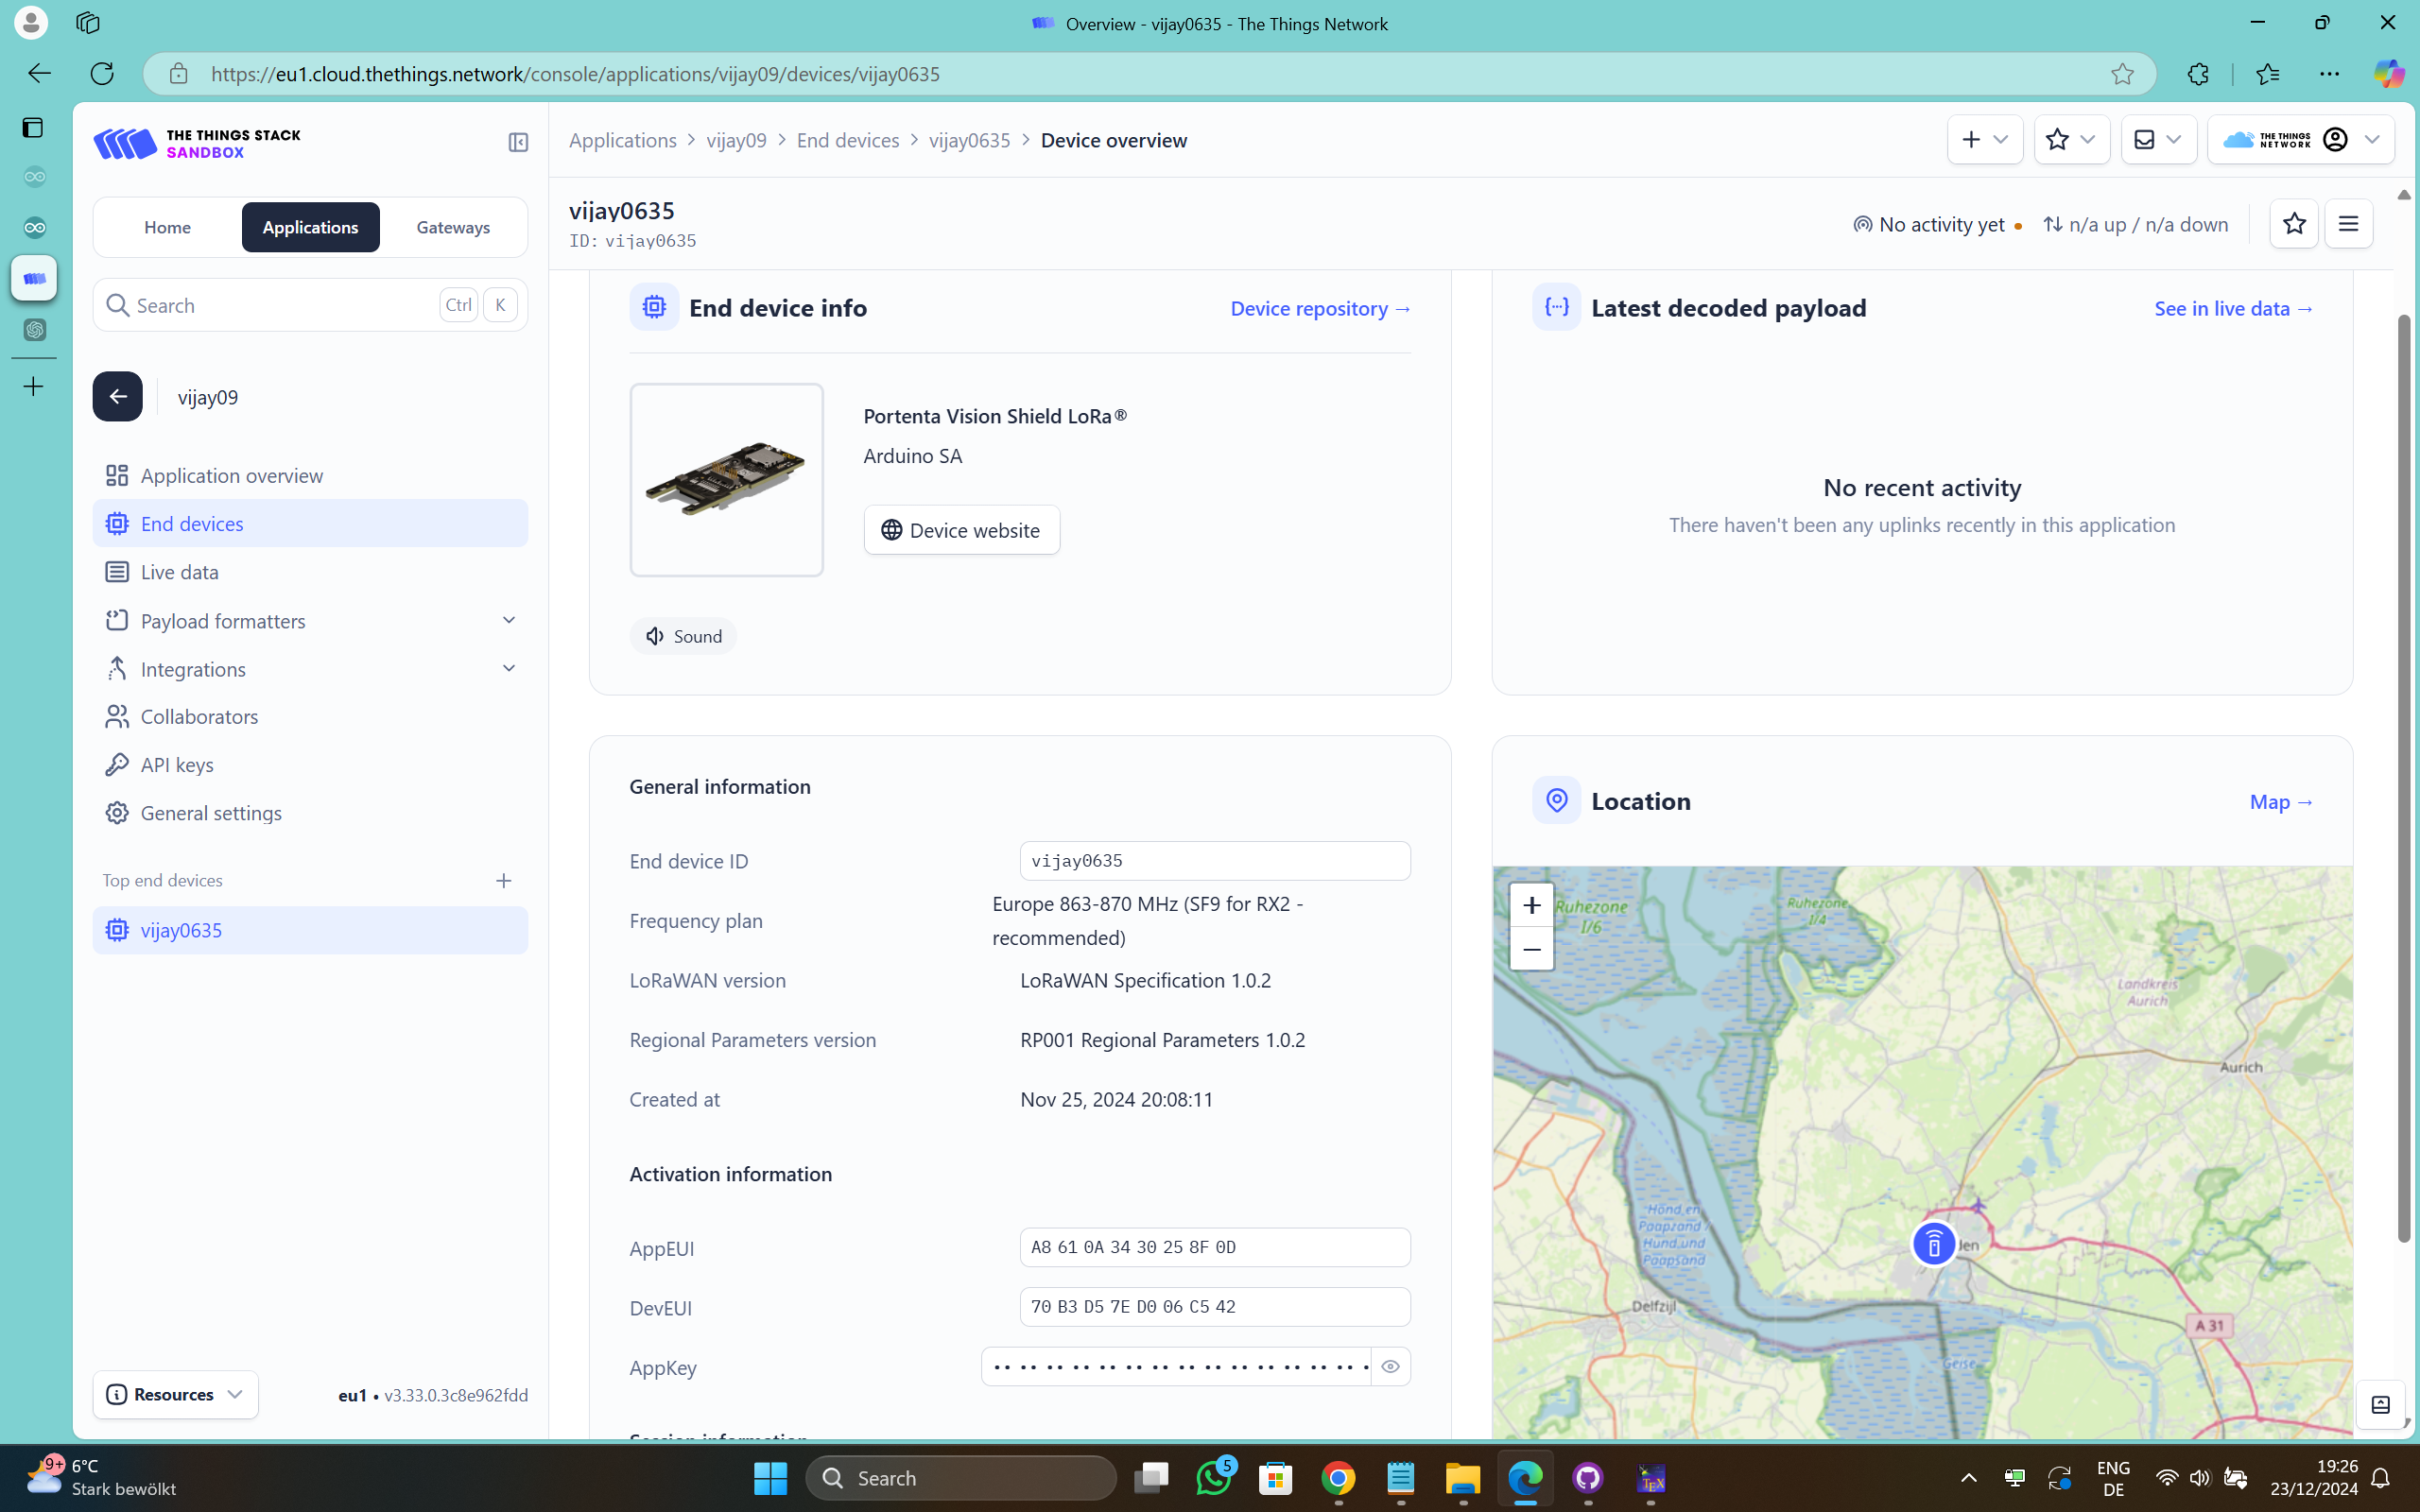
\includegraphics[width=0.7\linewidth]{Images/LORA/TTN.png}
				\caption{TTN}
				\label{TTN} 
			\end{center}
		\end{figure}




\section{Tests}

\subsection{Connecting the Portenta Vision Shield to TTN Using LoRa}
\label{LORAWAN}
This example explains how to connect your Portenta H7 to The Things Network (TTN) using the the Portenta Vision Shield's LoRa Connectivity feature. \cite{ArduinoTTN:2024}

\subsubsection{Overview}
This example explains how to connect your Portenta H7 to The Things Network (TTN) using the the Portenta Vision Shield's LoRa Connectivity feature. A data communication channel will be enabled between the H7 and a TTN application that will be configured on your TTN console. \cite{ArduinoTTN:2024}
\begin{comment}
	\subsubsection{Required Hardware and Software}
	
	\paragraph{Portenta H7}
	\begin{itemize}
		\item \textbf{Dual-core MCU:}
		\begin{itemize}
			\item Cortex-M7 (480 MHz) for high-performance tasks.
			\item Cortex-M4 (240 MHz) for low-power operations.
		\end{itemize}
		\item \textbf{Connectivity:} Supports Wi-Fi, Bluetooth, and LoRa via the Vision Shield.
		\item \textbf{Supports Edge AI and Machine Learning.}
		\item \textbf{Interface:} Includes SPI for communication.
	\end{itemize}
	
	\paragraph{Portenta Vision Shield – LoRa}
	\begin{itemize}
		\item \textbf{LoRa Module:} RAK4630 (Semtech SX1262 LoRa transceiver).
		\item \textbf{Onboard Camera:} Enables AI-powered image processing.
		\item \textbf{Audio Interface:} Includes two microphones for sound analysis.
	\end{itemize}
	
	\paragraph{U.FL Antenna}
	\begin{itemize}
		\item Essential for proper LoRa signal transmission and reception.
		\item Connects to the Vision Shield's LoRa module.
	\end{itemize}
	
	\paragraph{Arduino IDE 1.8.13+}
	\begin{itemize}
		\item Required for programming the Portenta H7 and the LoRa module on the Vision Shield.
		\item Needs additional board support via the Arduino mbed OS Portenta core.
	\end{itemize}
	
	\paragraph{The Things Network (TTN) Account}
	\begin{itemize}
		\item Required to register the Portenta H7 and enable LoRa communication.
		\item Visit \texttt{https://www.thethingsnetwork.org/} to create an account.
	\end{itemize}
\end{comment}

\subsubsection{Required Hardware and Software}

\begin{enumerate}
	\item Portenta H7
	\item Portenta Vision Shield - LoRa
	\item U.FL Antenna for Portenta H7 
	\item Arduino IDE 1.8.10+, Arduino IDE 2.0+, or the Arduino Cloud Editor
	\item USB-C Cable
	\item An Account with The Things Network \cite{ArduinoTTN:2024}
\end{enumerate}


\subsubsection {Installing the LoRa Module Firmware}
To be able to use the LoRa functionality, we need to first Install the firmware on the LoRa modem. This can be done through Arduino IDE by running a sketch included in the examples from the MKRWAN library.

\begin{enumerate}
	\item Connect the Portenta H7 and the Portenta Vision Shield - LoRa to your computer and open the Arduino IDE. 
	\item Install/update the \SHELL{MKRWAN} library from Arduino IDE menu \SHELL{Tools > Manage Libraries}[Refer figure ~\ref{Install MKRWAN}]. Type "MKRWAN" to find the library and click 'Install' or 'Update' if necessary. This library provides all the APIs to communicate with LoRa and LoRaWAN networks.
	\item Open the MKRWANFWUpdate standalone sketch from the Arduino IDE menu: \SHELL{File > Examples > MKRWAN}.(Refer figure ~\ref{MKRWAN Standalone})
	\item Upload the sketch. \cite{ArduinoTTN:2024}
\end{enumerate}

\begin{figure}
	\begin{center}
		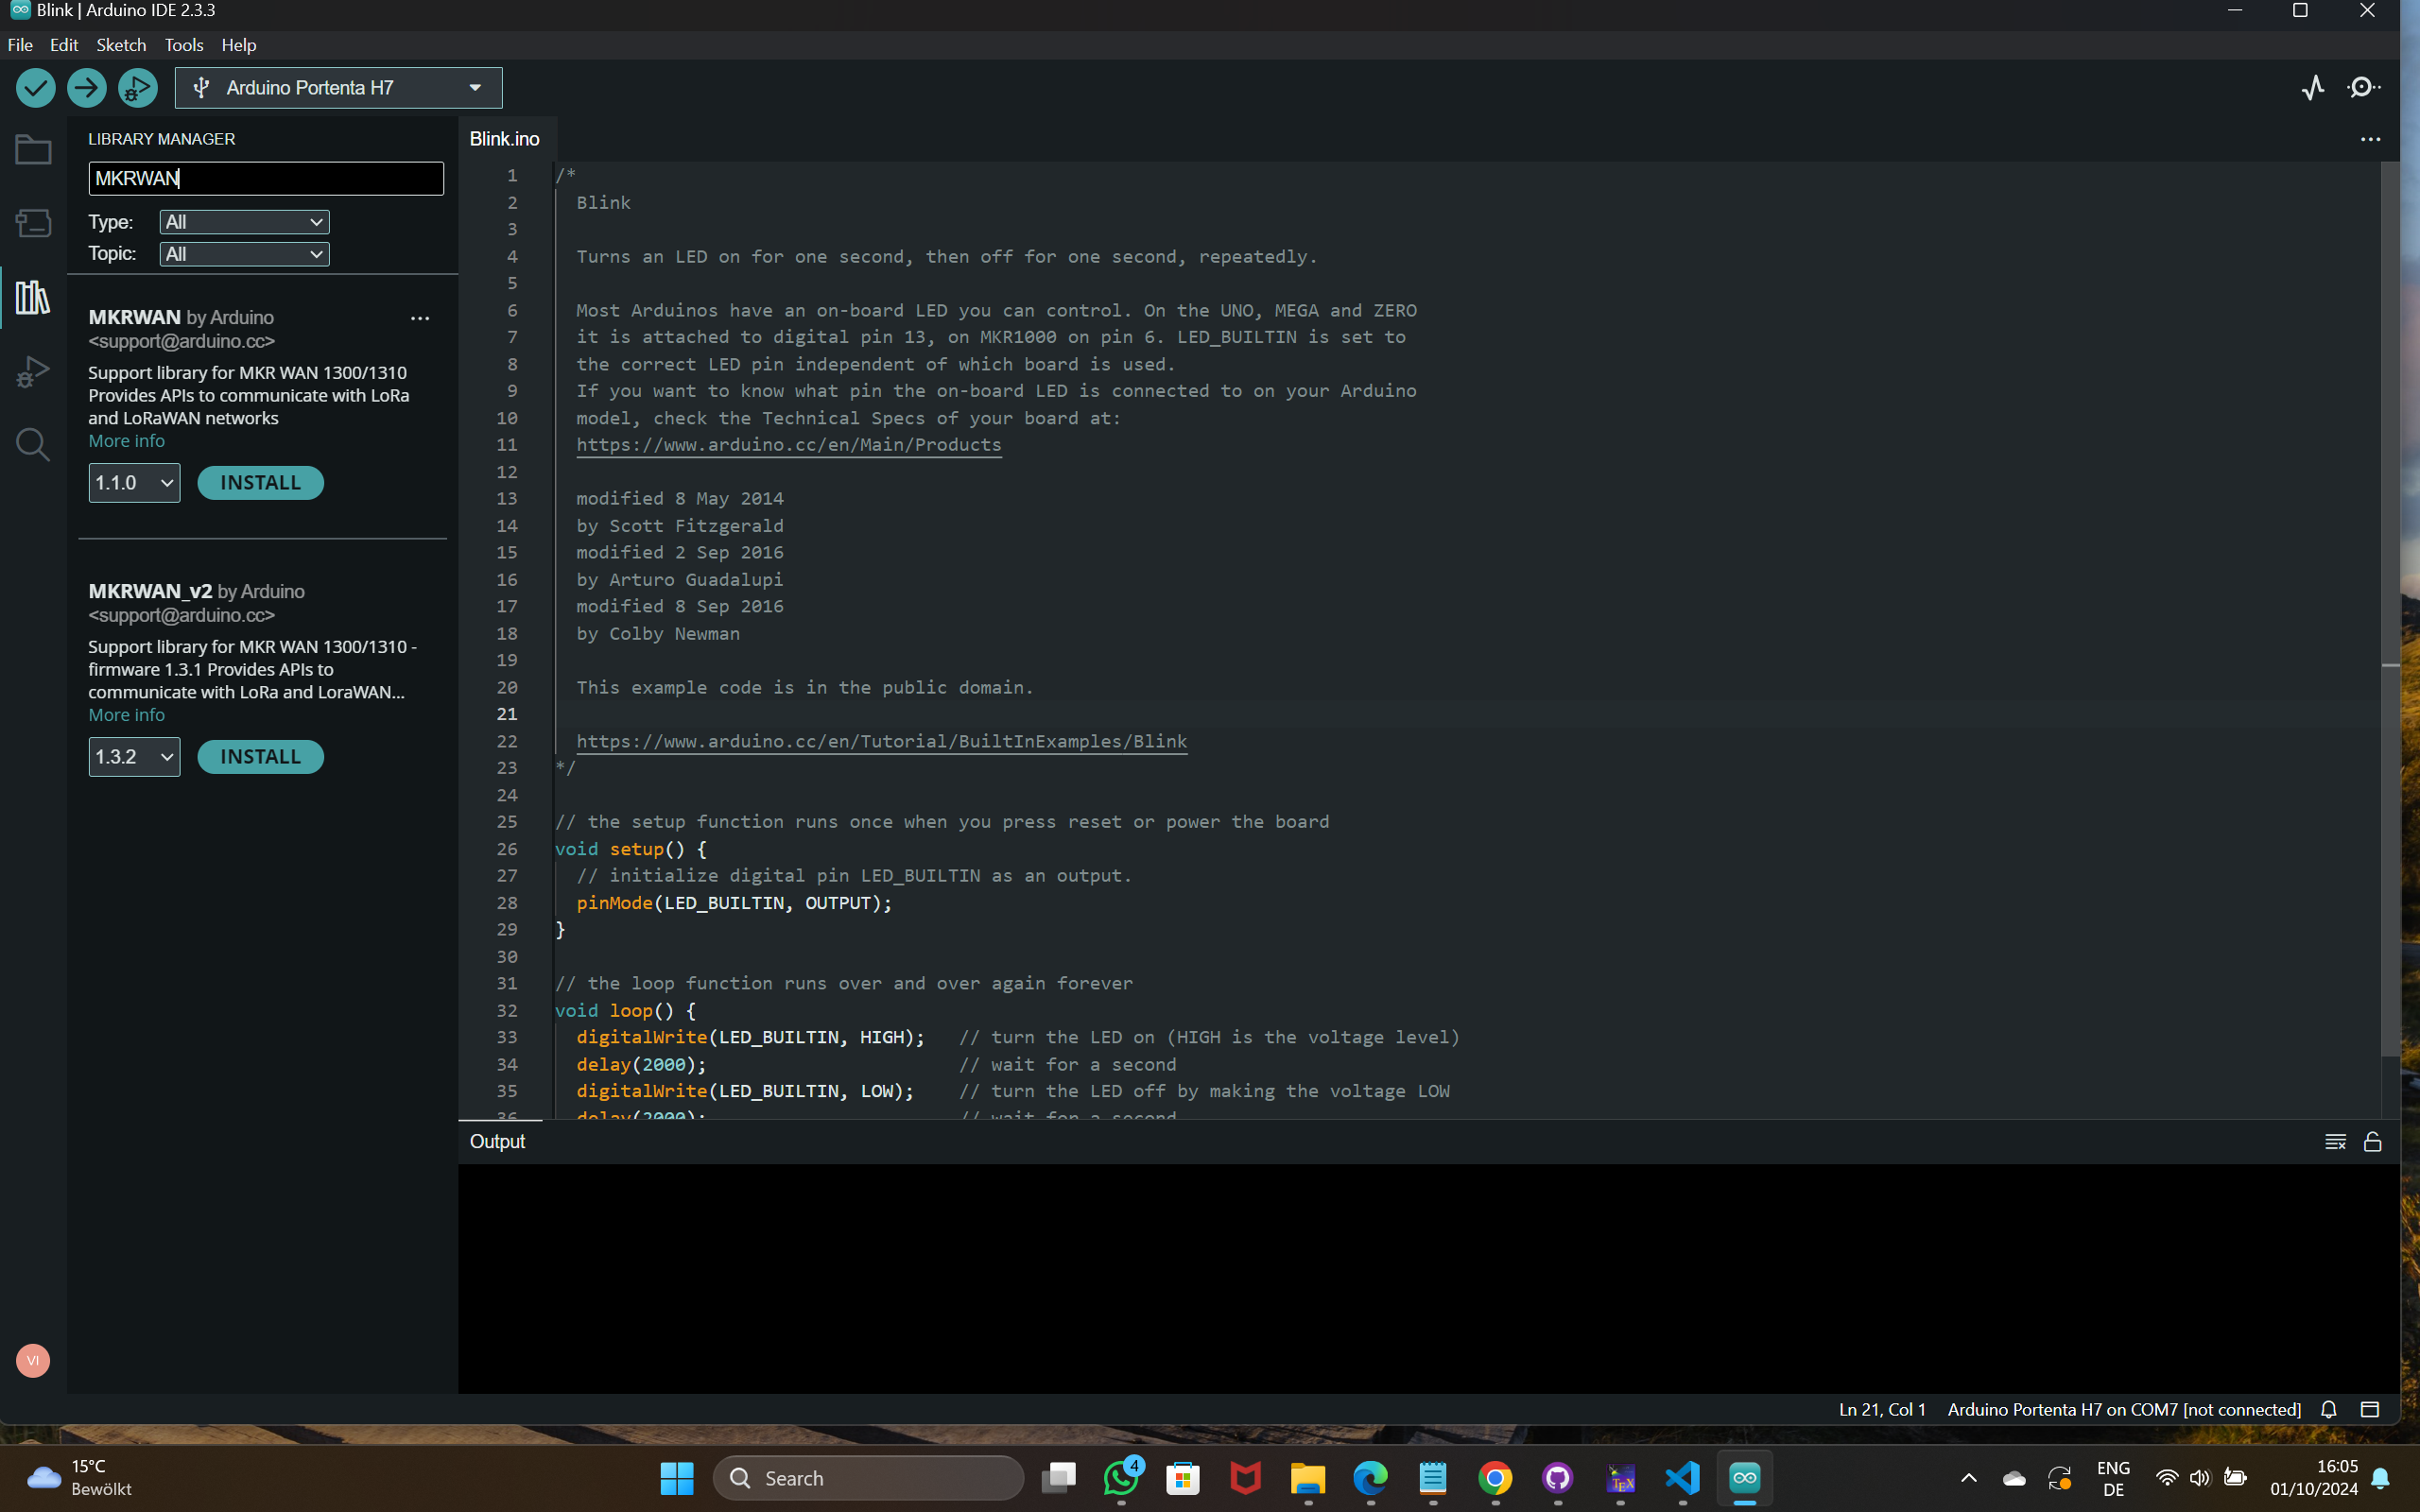
\includegraphics[width=0.7\linewidth]{Images/LORA/InstallMKRWAN.png}
		\caption{Install MKRWAN}
		\label{Install MKRWAN}
	\end{center}
\end{figure}

\begin{figure}
	\begin{center}
		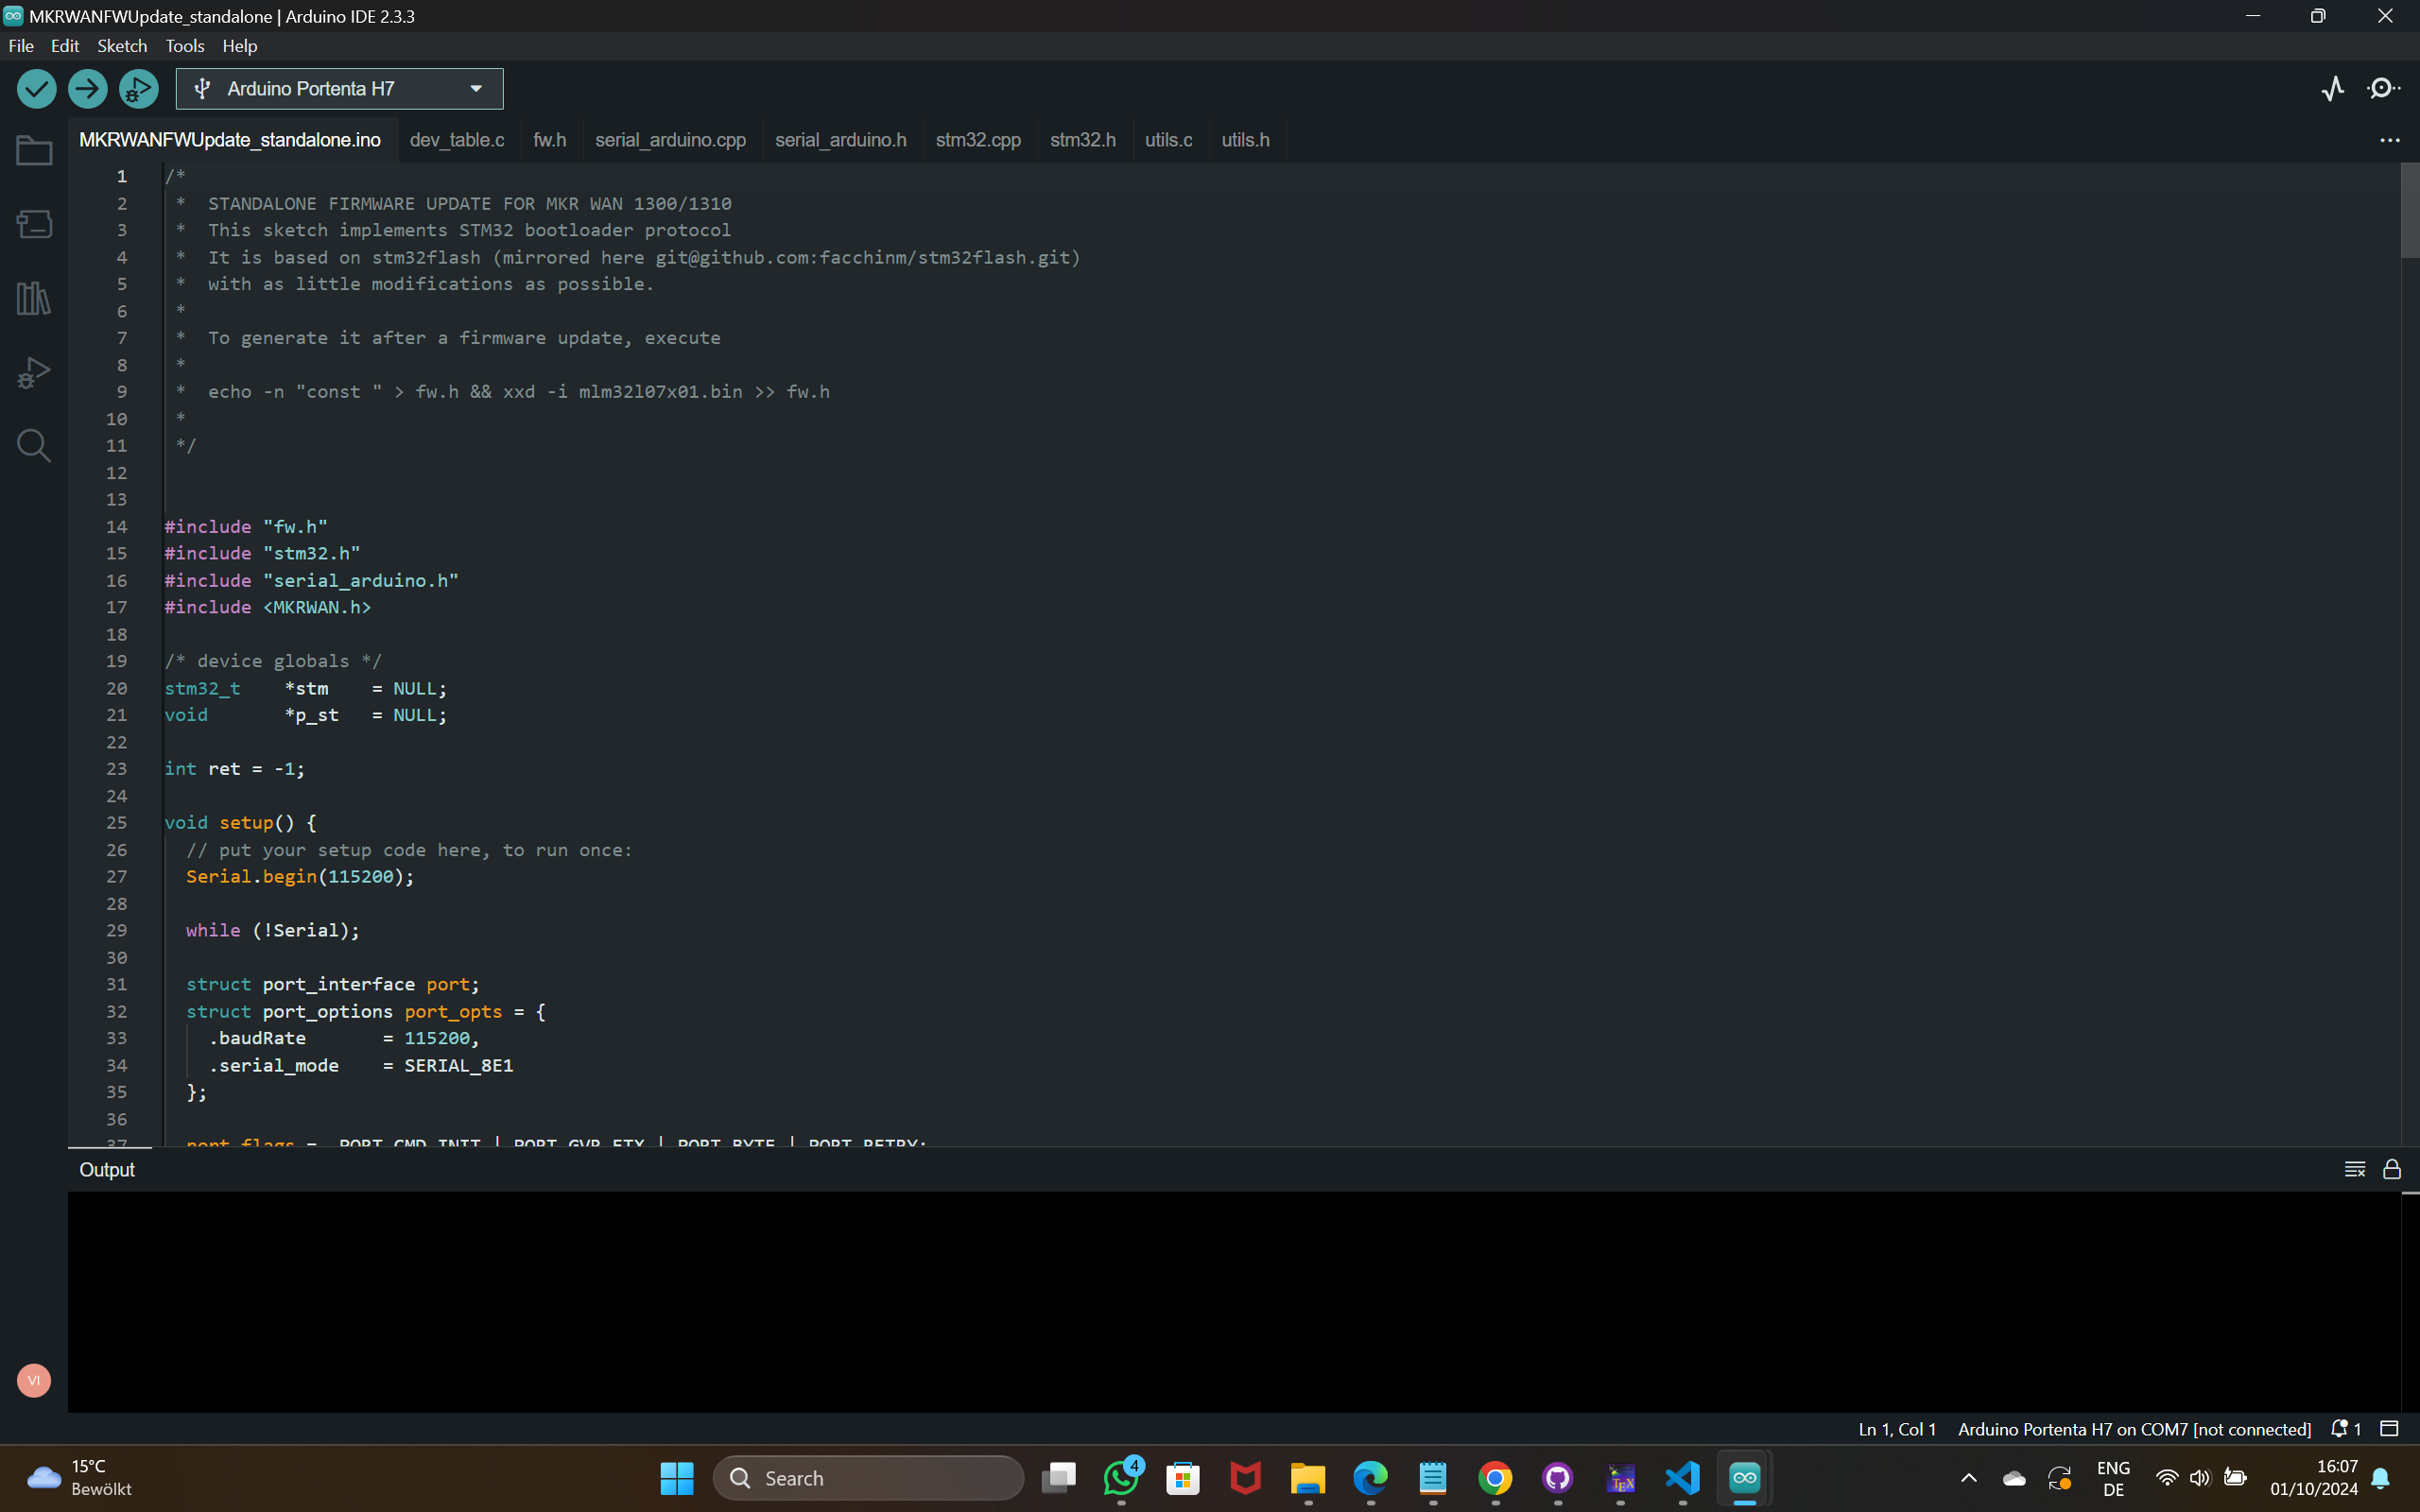
\includegraphics[width=0.7\linewidth]{Images/LORA/MKRWANStandalone.png}
		\caption{MKRWAN Standalone}
		\label{MKRWAN Standalone}
	\end{center}
\end{figure}

Open the Serial Monitor and wait for the update to be confirmed.(Refer figure ~\ref{SerialMonitor})

\begin{figure}
	\begin{center}
		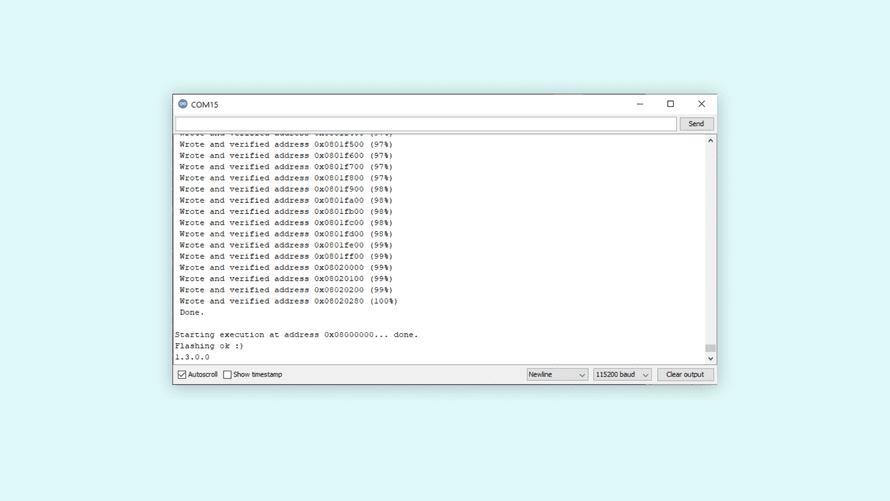
\includegraphics[width=0.7\linewidth]{Images/LORA/SerialMonitor.png}
		\caption{SerialMonitor}
		\label{SerialMonitor}
	\end{center}
\end{figure}



\subsubsection{Connecting to TTN} Once your board has been registered you can send information to TTN. Let's come back to the Serial Monitor and proceed. It will ask for: (Refer figure ~\ref{Select-board-h7})
		
		\begin{enumerate}
			\item Activation mode (that, in this case, is OTAA),
			\item The Application EUI
			\item The App Key.
		\end{enumerate}
		
		Lets start by making a connection Over-The-Air (OTA). Enter "1" in the Serial Monitor input box and press ENTER. Then, find the EUI and the App key from TTN \SHELL{Device Overview} page. You can read more into OTA vs ABP activation mode here.
		
		\begin{lstlisting}[language=C++, frame=single, numbers=left, basicstyle=\ttfamily\small]
			Your module version is: ARD-078 1.1.9
			Your device EUI is: a8xxxxxxxxxxxx0a
			Are you connecting via OTAA (1) or ABP (2)?
			Enter your APP EUI
			Enter your APP KEY
		\end{lstlisting}
		
		Next, introduce the APP EUI and the APP KEY in the Serial Monitor. If this process is done successfully, you will see this message: \cite{ArduinoTTN:2024}
		
		\begin{lstlisting}[language=C++, frame=single, numbers=left, basicstyle=\ttfamily\small]
			Message sent correctly!
		\end{lstlisting}
		
		else,
		
		\begin{figure}
			\begin{center}
				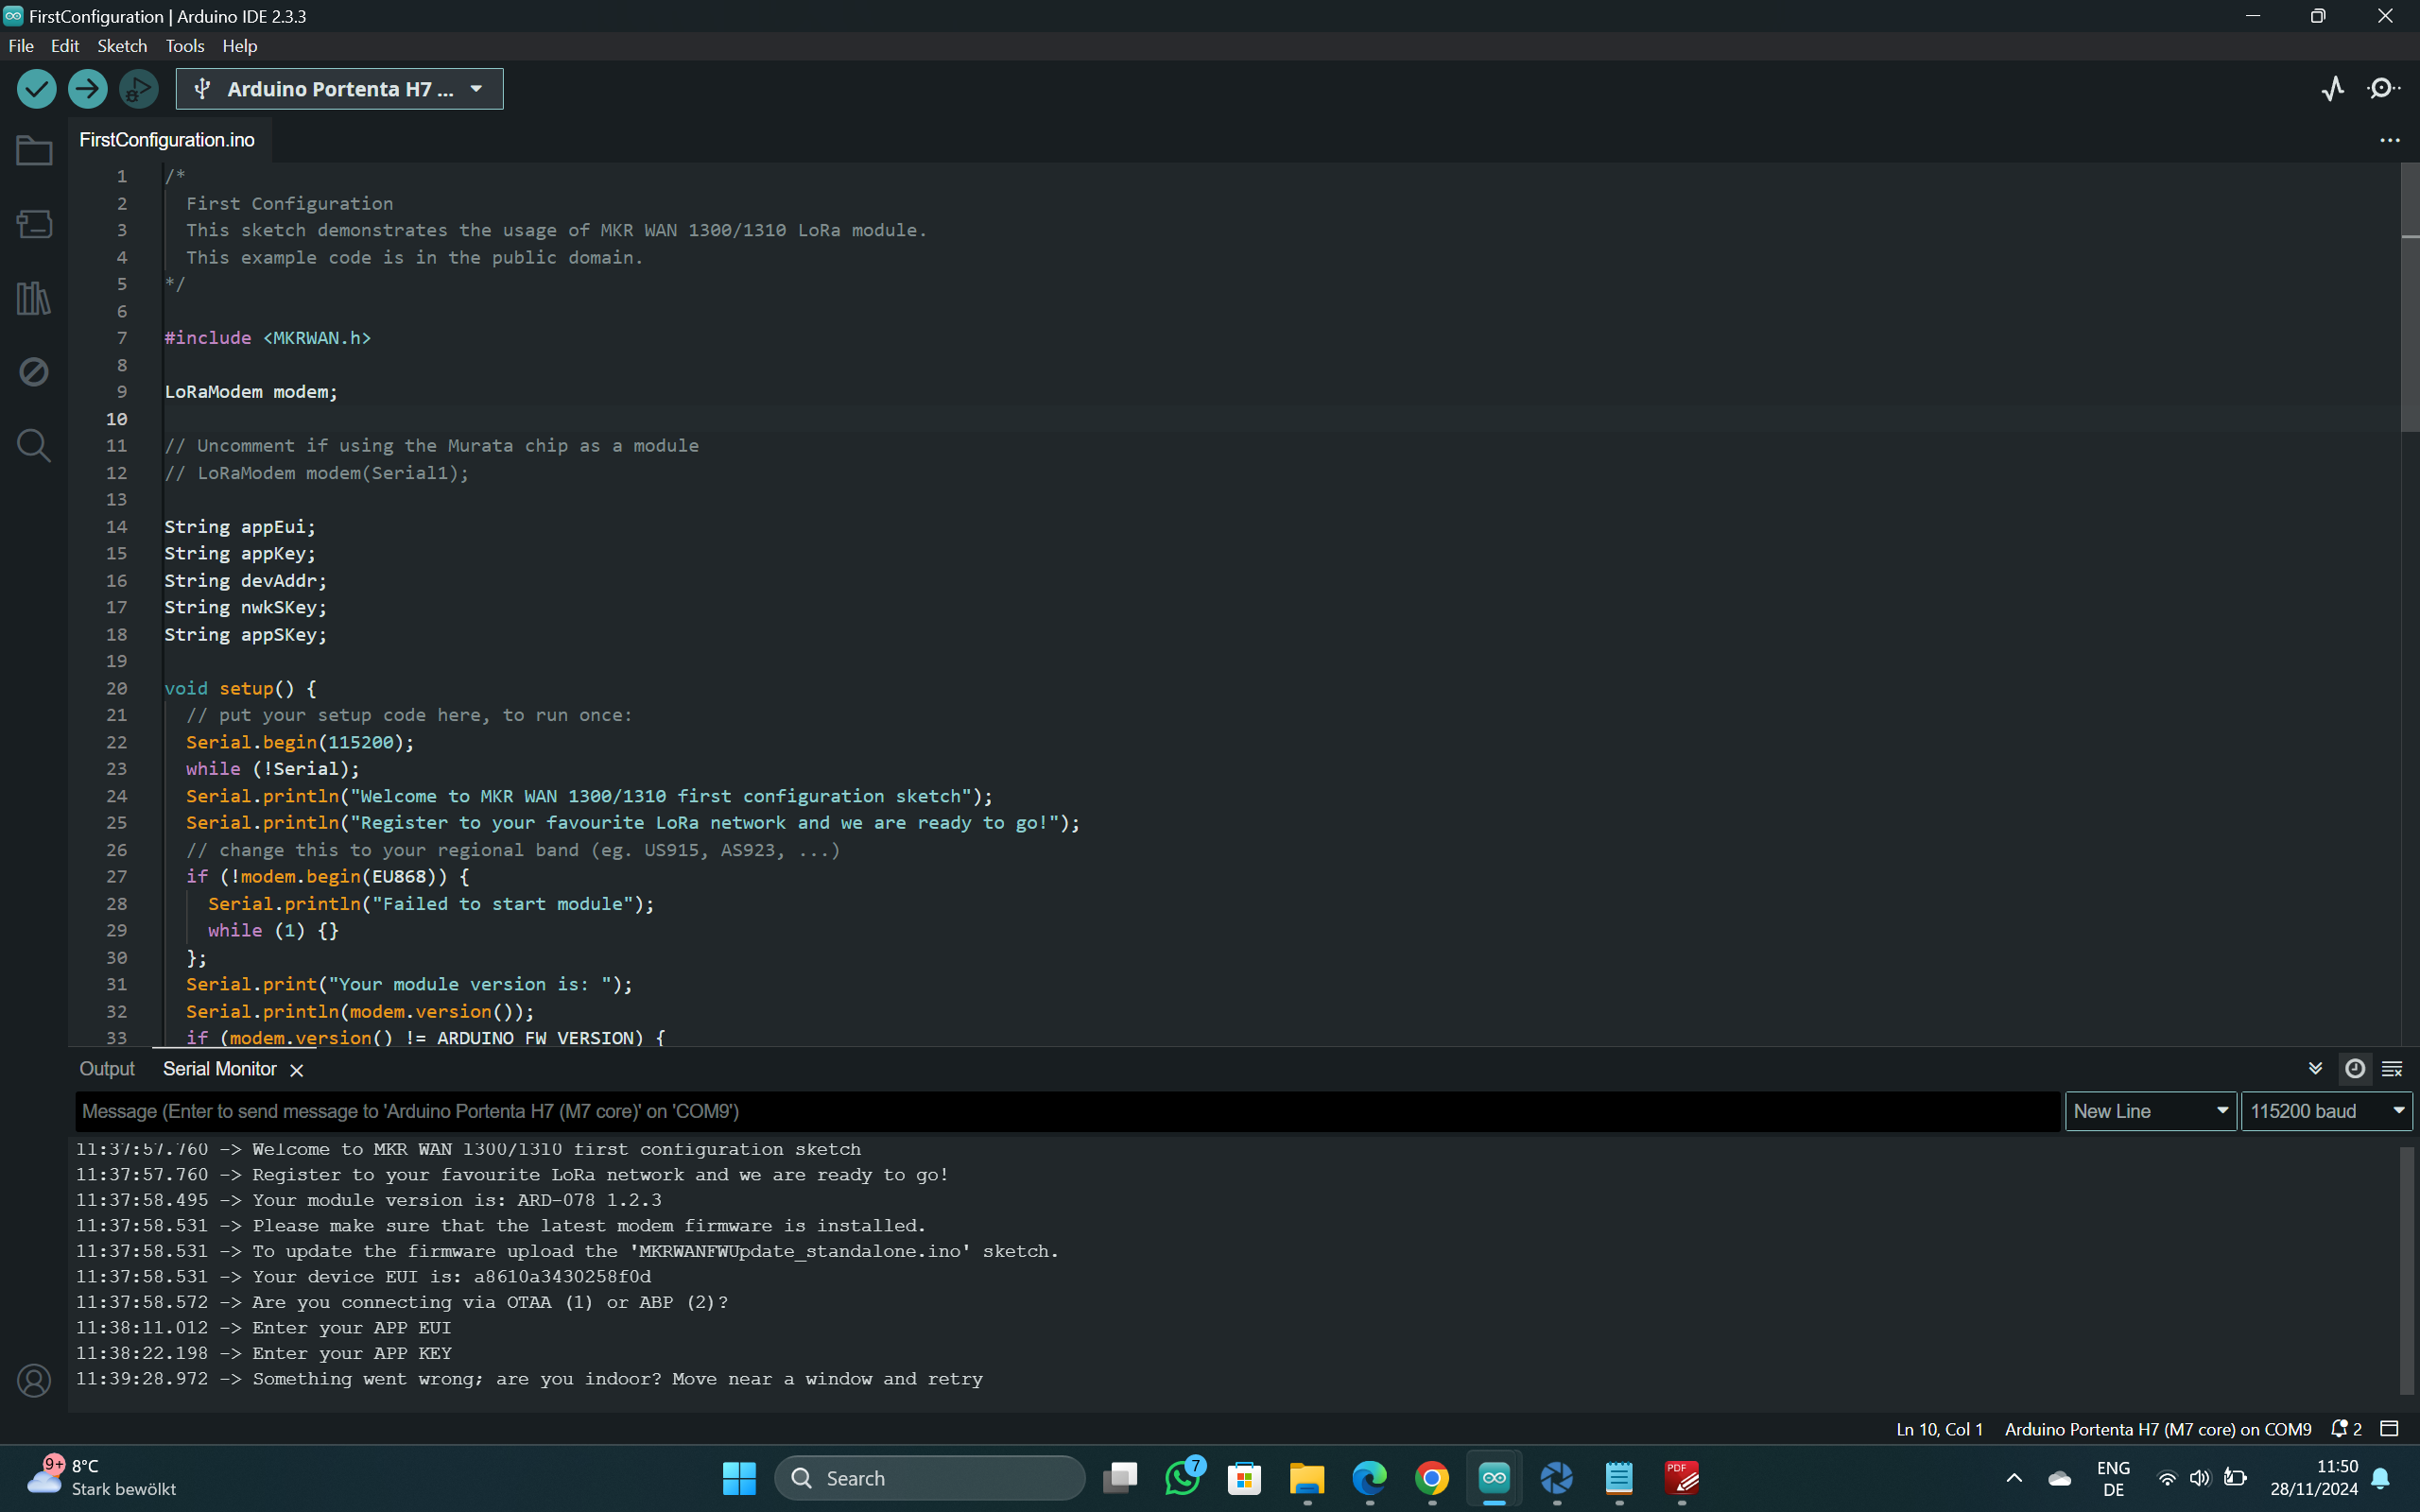
\includegraphics[width=0.7\linewidth]{Images/LORA/LoraConnection.png}
				\caption{Monitor Output}
				\label{Monitor}
			\end{center}
		\end{figure}
		
		\item \textbf{6. Conclusion:} If you receive this message, you have managed to configure the Portenta H7 and the Portenta Vision Shield - LoRa on TTN.
		
		You have retrieved the device EUI, used it to register the device in the TTN console, and programmed the board using the data provided by TTN. Now, you can send data over the LoRa network which can be viewed from anywhere in the world (as long as we have an Internet connection and your device is in the range of a TTN gateway). \cite{ArduinoTTN:2024}
		
	\end{itemize}
	
	


\subsection{Designing a Double LoRa Connectivity for the Arduino Portenta H7}
\label{P2P}

 Machine learning (ML) is nowadays deployed in ever smaller
computing devices including microcontrollers found in Internet
of Things (IoT) nodes [1]. Signal processing and ML tasks
are performed directly at the IoT device, communicating only
the result of a classification to remote gateways instead of the
raw data [2].
LoRa is a popular communication technology for the IoT.
LoRa links can cover several km of distance between the end
node, which produces the data, and the gateway. Most IoT
applications that use LoRa apply the LoRaWAN architecture
[3]. This architecture builds a star topology which establishes a
single hop between the end nodes and the gateway. LoRaWAN,
however, does not directly interconnect the end nodes between
themselves. \cite{PortentaLANMAN2022}
\newline
LoRa mesh networks have been proposed for diverse sce
narios which cannot be addressed well by the LoRaWAN
architecture [4]. For geographically spread IoT nodes and
low gateway density, multi-hop LoRa can be used where
intermediate nodes operate as repeaters that broadcast traffic
to other LoRa nodes to finally reach a gateway [5]. Another
scenario are gateway-less applications such as Meshtastic [6].
In this real application the nodes communicate only within the
LoRa mesh network, without any gateway to the Internet.
Given the potential of LoRa mesh networks, in this paper
we investigate the possibility of the Arduino Portenta H7 for
becoming a node of a LoRa mesh network. The Portenta H7 is
a recent microcontroller board which targets high performance
 industrial machine learning applications, being equipped for
this with a dual core and very complete on-board sensors. We
focus on the Portenta’s LoRa connectivity challenge given that
the board in practical applications has already been shown
to be well prepared for running embedded machine learning
applications \cite{PortentaLANMAN2022}\newline

\subsubsection{DESIGN}

\textbf{A: Analysis of the Arduino LoRa Vision Shield}\newline

The Arduino Portenta H7 is a board with two cores, a
Cortex M7 running at 480 MHz and a Cortex M4 running
at 240 MHz, to which shields can be connected in order
to extend the board with additional features such as sensors(Refer figure ~\ref{LoRAConnectivity}).
The shield which provides LoRa connectivity is the Arduino
Portenta LoRa Vision Shield2. This shield contains the Murata
CMWX1ZZABZ-078 module3, which is internally composed
of the SX1276 LoRa radio chip from Semtech, together with
other elements for signal modulation, reception and transmis
sion and the STM32L0 microcontroller. \cite{PortentaLANMAN2022}
\newline
Our aim is to analyze if the Arduino Portenta LoRa Vision
Shield supports RadioLib4, a popular communication library
which allows to implement LoRa point-to-point communi
cations. From analyzing the Murata datasheet we observed,
however, that even though the module has SPI connectivity,
it is not physically implemented in the Arduino Portenta
Vision Shield and therefore the Arduino Portenta H7 cannot
communicate directly with the Murata’s SX1276 LoRa radio
through this communication protocol. This fact disables the
use of RadioLib which does require the SPI communication.
While we found that the use of RadioLib was not possible,
the MKRWANlibrary is officially compatible with the Portenta
LoRa Vision Shield. Using the MKRWAN library we observed
that this library communicates with the Murata module over
AT commands, which allows to manage the LoRaWAN con
nectivity of the radio. For operating AT commands, the serial
bus named UART8 in the Portenta Vision Shield is connected
to the pins named Serial3 of the Portenta board. Therefore, the
firmware implemented in the Murata module requires the radio
to be connected to a LoRaWAN network. However, with AT
commands as the only access to the module,it is not possible to
conduct operations below the LoRaWAN layer,which is needed
when we want to use the radio in a LoRa mesh network. In
addition, it was pointed out that the current implementation
of the MKRWAN library does not support some relevant AT
commands. \cite{PortentaLANMAN2022} \newline

\textbf{B. The choice of the double LoRa connectivity}\newline

Our analysis reveled that while the Murata firmware supports
LoRaWAN, it does not allow to operate on the layer below to
manage basic LoRa packets. There have been efforts by the
community to replace the Murata firmware, but the result is
experimental and there is no official support for the Portenta
LoRa Vision Shield6,
We therefore chose the option to connect a second LoRa
radio to the Arduino Portenta H7 and connect it as shown in
Figure ~\ref{LCommunication}. The SCK, MISO, MOSI and CS signal connections
belong to the SPI protocol. In addition, the connection with
the SX1276 requires the interrupt and reset signals to correctly
handle sending and receiving messages (INT and RST signals,
respectively). \cite{PortentaLANMAN2022} \newline

\begin{figure}
	\begin{center}
		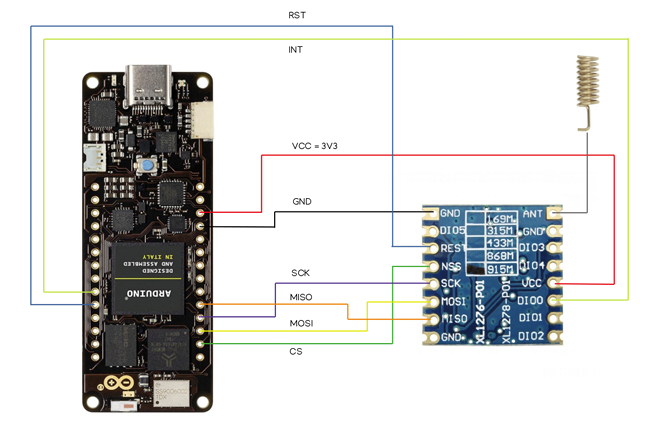
\includegraphics[width=0.7\linewidth]{Images/LORA/LoRAConnectivity.png}
		\caption{Connection for SX1276 chip to the Arduino Portenta H7}
		\label{LoRAConnectivity} 
	\end{center}
\end{figure} 

\textbf{III. LIBRARY COMPATIBILITY}\newline

 In order to validate the design, we first aim to verify that the
new LoRa radio added to the Portenta supports the Arduino
LoRa library7. We flash existing code fragments for LoRa
sender and receiver to two Portenta H7 boards and could verify
the successful communication between the two boards using
the added LoRa radio.
The second test aims to validate that RadioLib can be used.
With the additional LoRa radio board the SPI interface required
by RadioLib is available. It needs to be mentioned that in order
 to use RadioLib, another interrupt signal has to be added by
physically connecting the Portenta H7 with the DIO1 signal
of the radio board, which finalizes the reception timer. Using
a LoRa sender and receive code the communication between
two Portenta boards over the added LoRa radio using RadioLib
could be verified. An OLED display was used to verify the
successful communication. \cite{PortentaLANMAN2022}\newline

\begin{figure}
	\begin{center}
		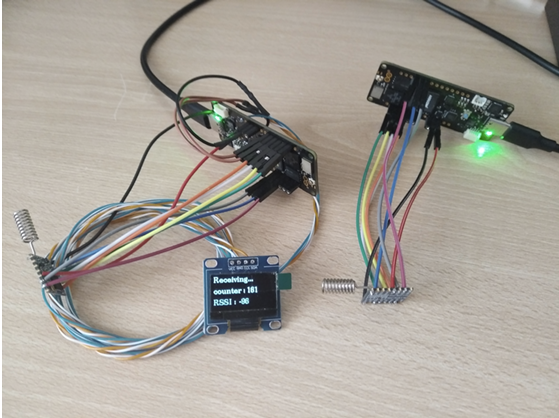
\includegraphics[width=0.7\linewidth]{Images/LORA/LCommunication.png}
		\caption{Communication test of two Arduino Portenta H7 by LoRa}
		\label{LCommunication} \cite{PortentaLANMAN2022}
	\end{center}
\end{figure}

\textbf{IV. CONCLUSIONS AND OUTLOOK} \newline

We designed a double LoRa connectivity for the Arduino
Portenta H7 to enable this board to become part of a LoRa mesh
network. The new design extends the board’s application to
scenarios in which the device not only reaches the LoRaWAN
gateway, but can also be part of a LoRa mesh network.
In future work we aim to integrate the new communication
capacity into the Mbed OS available for the Arduino Portenta
H7 and use it for interconnected machine learning applications. \cite{PortentaLANMAN2022} \newpage




\subsection{LoRaWAN vision with Edge Impulse and Portenta H7}

This is an example application that runs a computer vision model on the Portenta H7 and streams the results over LoRaWAN. The application uses the camera on the Portenta Vision Shield in combination with a machine learning model trained in Edge Impulse to determine when an interesting event happens, then sends this using the LoRa radio on the Portenta Vision Shield back to the network. \cite{edge_impulse_portenta_lorawan:2025} \newline 


\subsubsection{Required Hardware and Software}

\begin{enumerate}
	\item Portenta H7
	\item Portenta Vision Shield - LoRa
	\item U.FL Antenna for Portenta H7 
	\item Arduino IDE 1.8.10+, Arduino IDE 2.0+, or the Arduino Cloud Editor
	\item USB-C Cable
	\item An Account with The Things Network \cite{edge_impulse_portenta_lorawan:2025}
\end{enumerate}

This firmware integrates the Portenta H7 board with the Vision Shield (LoRa) for Edge Impulse-based machine learning and LoRaWAN communication. Below is a breakdown of the code: \cite{edge_impulse_portenta_lorawan:2025}

\subsubsection{Header Files and Dependencies}

\begin{lstlisting}[language=C++, caption=Included Header Files]
	#include "ei_main.h"
	#include "ei_device_portenta.h"
	#include "porting/ei_classifier_porting.h"
	#include "ei_portenta_fs_commands.h"
	#include "ei_microphone.h"
	#include "ei_config_types.h"
	#include "at_cmd_repl_mbed.h"
	#include "ei_run_impulse.h"
	#include "sensors/ei_camera.h"
	#include <MKRWAN.h>
\end{lstlisting}

These headers provide support for:
\begin{itemize}
	\item Edge Impulse functionalities for AI/ML model inference.
	\item LoRaWAN communication via \texttt{MKRWAN.h}.
	\item AT command handling for serial communication.
\end{itemize}

\subsubsection{LoRa Modem and LED Initialization}

\begin{lstlisting}[language=C++, caption=LoRa Modem and LED Setup]
	LoRaModem modem;
	mbed::DigitalOut led(LED1);
\end{lstlisting}

\begin{itemize}
	\item \texttt{LoRaModem modem;} - Initializes the LoRa modem.
	\item \texttt{led(LED1);} - Controls the onboard LED.
\end{itemize}

\subsubsection{AT Command Interpreter Setup}

\begin{lstlisting}[language=C++, caption=AT Command Interpreter Setup]
	EventQueue main_application_queue;
	static unsigned char repl_stack[8 * 1024];
	static AtCmdRepl repl(&main_application_queue, ei_get_serial(), sizeof(repl_stack), repl_stack, 5);
\end{lstlisting}

This initializes:
\begin{itemize}
	\item An event queue for managing background tasks.
	\item AT Command REPL (Read-Eval-Print-Loop) for serial interactions.
\end{itemize}

\subsubsection{LoRaWAN Credentials}

\begin{lstlisting}[language=C++, caption=LoRaWAN Credentials]
	static String appEui = "70B3D57ED003BFCA";
	static String appKey = "1F537E0DDCFCFF43443004F3A88C4294";
\end{lstlisting}

These credentials authenticate the device with The Things Network (TTN).

\subsubsection{Memory Allocation Function}

\begin{lstlisting}[language=C++, caption=Memory Allocation]
	void fill_memory() {
		size_t size = 8 * 1024;
		size_t allocated = 0;
		while (1) {
			void *ptr = ei_malloc(size);
			if (!ptr) {
				if (size == 1) break;
				size /= 2;
			}
			else {
				allocated += size;
			}
		}
		ei_printf("Allocated: %u bytes\n", allocated);
	}
\end{lstlisting}

This function tests available RAM by attempting allocations in 8KB chunks.

\subsubsection{LoRaWAN Connection and Data Transmission}

\begin{lstlisting}[language=C++, caption=LoRaWAN Connection]
	void lorawan_main() {
		ei_printf("Hello from the LoRaWAN thread...\n");
		ThisThread::sleep_for(5000);
		
		if (!modem.begin(EU868)) {
			ei_printf("Failed to initialize modem\n");
		}
		
		ei_printf("[LRWN] Device EUI is: %s\n", modem.deviceEUI().c_str());
		
		bool connected = false;
		while (!connected) {
			ei_printf("[LRWN] Joining network...\r\n");
			connected = modem.joinOTAA(appEui, appKey);
			if (connected) {
				ei_printf("[LRWN] Joined network!\r\n");
			}
			else {
				ei_printf("[LRWN] Joining network failed, retrying in 10 seconds...\r\n");
			}
			ThisThread::sleep_for(10000);
		}
	}
\end{lstlisting}

This function:
\begin{itemize}
	\item Connects the device to TTN using Over-The-Air Activation (OTAA).
	\item Retries every 10 seconds if the connection fails.
\end{itemize}

\subsubsection{Sending AI Inference Results via LoRa}

\begin{lstlisting}[language=C++, caption=Sending AI Events via LoRa]
	while (1) {
		if (is_event_changed && ei_read_timer_ms() - last_message_sent >= 7000) {
			if (strcmp(last_event, "uncertain") == 0 || strcmp(last_event, last_message_str) == 0) {
				ThisThread::sleep_for(1000);
				continue;
			}
			
			ei_printf("[LRWN] Sending event: '%s'\n", last_event);
			modem.dataRate(5);
			modem.setPort(3);
			modem.beginPacket();
			modem.print(last_event);
			int err = modem.endPacket(false);
			ei_printf("[LRWN] Sending event: '%s' returned %d\n", last_event, err);
			
			memcpy(last_message_str, last_event, 31);
			last_message_sent = ei_read_timer_ms();
			is_event_changed = false;
		}
		ThisThread::sleep_for(1000);
	}
\end{lstlisting}

This transmits detected events over LoRa every 7 seconds, ignoring uncertain classifications.

\subsubsection{Running Edge Impulse Model}

\begin{lstlisting}[language=C++, caption=Executing Edge Impulse Model]
	void run_nn_at() {
		ei_at_cmd_handle("AT+RUNIMPULSE");
	}
\end{lstlisting}

This function executes the Edge Impulse ML model when triggered via AT command.

\subsubsection{Main Execution Flow (ei\_main)}

\begin{lstlisting}[language=C++, caption=Main Execution Function]
	void ei_main() {
		ei_sleep(1000);
		
		ei_printf("Hello from Edge Impulse Device SDK.\r\n"
		"Compiled on %s %s\r\n", __DATE__, __TIME__);
		
		ei_portenta_fs_init();
		ei_camera_init();
		
		ei_at_register_generic_cmds();
		ei_at_cmd_register("RUNIMPULSE", "Run the impulse", run_nn_with_cb);
		ei_at_cmd_register("RUNIMPULSEDEBUG", "Run the impulse", run_nn_debug_with_cb);
		ei_at_cmd_register("FILLMEMORY", "Fill memory", fill_memory);
		
		Thread lorawan_thread;
		lorawan_thread.start(&lorawan_main);
		
		EiDevice.set_state(eiStateIdle);
		repl.start_repl();
		main_application_queue.dispatch_forever();
	}
\end{lstlisting}

This initializes Edge Impulse, registers AT commands, starts the LoRaWAN thread, and enters the main event loop. \cite{edge_impulse_portenta_lorawan:2025}

\textbf{Full Code:}

\begin{code}
	The full project and source code are available here:  
	\url{https://github.com/edgeimpulse/example-portenta-lorawan/blob/master/src/ei_main.cpp}
\end{code}

\subsubsection{Conclusion}

This firmware:
\begin{itemize}
	\item Runs an Edge Impulse ML model for event detection.
	\item Connects to TTN over LoRaWAN.
	\item Sends detected events via LoRa.
	\item Supports AT command interaction. \cite{edge_impulse_portenta_lorawan:2025}
\end{itemize}






